
% ------------------ DOCUMENT SETUP ------------------ 
% The document class defines the document type (report) and sets the font size (10pt)
\documentclass{report}

% Optional math commands from https://github.com/goodfeli/dlbook_notation.
\input{math_commands.tex}
\author{James Chapman}

% Inputs the Document Packages
% ------------------ PACKAGES ------------------ 
% Packages add extra commands and features to your LaTeX document. 
% In here, some of the most common packages for a thesis document have been added 

% LaTeX's float package
\usepackage{float}

% LaTeX's color package
\usepackage{color}

% Add color to Tables
\usepackage[table,xcdraw]{xcolor}

% LaTeX's main math package
\usepackage{amsmath}
\usepackage{amsthm}
\newtheorem{thm}{Theorem}
\usepackage[ruled,vlined]{algorithm2e}
\usepackage{esvect}
\usepackage{tikz}
\usetikzlibrary{patterns}
\usetikzlibrary{bayesnet}
\usetikzlibrary{arrows}
\usepackage{graphicx}
\usepackage{caption}
\usepackage{subcaption}
\usetikzlibrary{backgrounds}
\usepackage{algorithmic}
\usepackage{hyperref}
\usepackage[capitalize,noabbrev]{cleveref}

% LaTeX's Caption and subcaption packages
\usepackage[format=hang,font=normalsize,labelfont=bf,labelsep=colon,singlelinecheck=off]{caption}
\usepackage{subcaption}

% The graphicx package provides graphics support for adding pictures.
\usepackage{graphicx}

% Longtable allows you to write tables that continue to the next page.
\usepackage{longtable}

% Font encoding
\usepackage[T1]{fontenc}

% This package allows the user to specify the input encoding
\usepackage[utf8]{inputenc}

% This package allows you to add empty pages
\usepackage{emptypage}

% Allows inputs to be imported from a directory
\usepackage{import}

% Provides control over the typography of the Table of Contents, List of Figures and List of Tables
\usepackage{tocloft}

% The setspace package controls the line spacing properties.
\usepackage{setspace}

% Allows the customization of Latex's title styles
\usepackage{titlesec}

% Allows the customization of Latex's table of contents title styles
\usepackage{titletoc}

% The package provides functions that offer alternative ways of implementing some LATEX kernel commands
\usepackage{etoolbox}

% Provides extensive facilities for constructing and controlling headers and footers
\usepackage{fancyhdr} 

% Typographical extensions, namely character protrusion, font expansion, adjustment 
%of interword spacing and additional kerning
\usepackage{microtype}

% Generates PDF bookmarks
\usepackage{bookmark}

% Use these two packages together -- they define symbols
%  for e.g. units that you can use in both text and math mode.
\usepackage{gensymb}
\usepackage{textcomp}

% Bibliography package
\usepackage[backend=biber,style=nature]{biblatex}
\addbibresource{References.bib} % Add the .bib file that contains the references

% This package provides an easy way to input latin sample text (for the template only)
\usepackage{blindtext}

\usepackage{amsfonts} 

% Controls how many subsections the document can take
%  and how many of those will get put into the contents pages.
\setcounter{secnumdepth}{2}
\setcounter{tocdepth}{2}

% Places a dot after Chapter/Section/Subsection number in Table of Contents
\renewcommand{\cftchapaftersnum}{.}
\renewcommand{\cftsecaftersnum}{.}
\renewcommand{\cftsubsecaftersnum}{.}

%  Customize Dot spacing in Table of Contents/List of Figures/Tables
\renewcommand{\cftdotsep}{0.3}

% Numeration Type for Chapters and Sections (Roman I, II, II / Arabic 1, 2, 3)
\renewcommand\thechapter{\Roman{chapter}}
\renewcommand\thesection{\arabic{section}}

% Formatting Table of Contents/Lists titles
\renewcommand{\contentsname}{\normalfont\bfseries\LARGE{CONTENTS}}
\renewcommand{\listfigurename}{\normalfont\bfseries\LARGE{LIST OF FIGURES}}
\renewcommand{\listtablename}{\normalfont\bfseries\LARGE{LIST OF TABLES}}


% Title Formatting customization
\titleformat{\chapter}{\normalfont\bfseries\LARGE}{\thechapter.}{1em}{\MakeUppercase}

\titleformat{\section}{\normalfont\bfseries\large}{\thesection.}{1em}{\MakeUppercase}
\titlespacing*{\section} {0pt} {15pt} {15pt} % left, before, after

\titleformat{\subsection}{\normalfont\bfseries\large}{\thesubsection.}{1em}{}
\titlespacing*{\subsection} {0pt} {10pt} {10pt}

\titleformat{\subsubsection}{\normalfont\bfseries\large}{}{1em}{}
\titlespacing*{\subsubsection} {0pt} {10pt} {10pt}


% HEADER AND FOOTER
\pagestyle{fancy}  % Set Page Style (Header and Footer Style)
\fancyhf{}  % Clears the header and footer (from the default info)

% Header
\renewcommand{\headrulewidth}{0pt}  % Removes the default Horizontal Line in Header
\fancyhead[L]{James Chapman}
\fancyhead[R]{January 2022}

% Footer
\fancyfoot[C]{\thepage} % Page Number

% Change figure numbering per section
\numberwithin{figure}{chapter}
\numberwithin{table}{section}






%  -------------------------------------------------
%  --------- The document starts from here --------- 
%  -------------------------------------------------

\begin{document}

% ------------------  TITLE PAGE -------------------
\begin{titlepage}
\begin{center}
    % Title
    {\LARGE\textbf{Towards Scalable, Flexible, and Interpretable Self-Supervised Learning from Multiview Biomedical Data}
\author{James Chapman\\
    % Subtitle
    \\}}

    \vspace{0.8cm}
    by\\
    \vspace{0.8cm}

    % Author
    {\LARGE\textbf{James Chapman\\}}
    % Date
    \vspace{1.5cm}
    {\LARGE\textbf{January 2022}}

    \vfill

    \textbf{\setstretch{2.0}       
    Upgrade Report\\
    \vspace{1cm}
    i4health CDT\\
    University College London\\}

    \vspace{2cm}
\end{center}
\end{titlepage}

\onehalfspacing

% ----------------------  ABSTRACT -----------------------
\newpage
\chapter*{Abstract} % the Asterix (*) indicates that this section will be added to the table of contents but no number will be present beside it.
% \addcontentsline{toc}{chapter}{Abstract}

Biomedical data are essential for advancing our knowledge and practice of medicine and healthcare. However, biomedical data are also challenging to analyze due to their complexity, heterogeneity, high-dimensionality, and scarcity of labels. To overcome these challenges, self-supervised learning (SSL) has emerged as a promising paradigm for learning from unlabeled data by leveraging inherent structures or patterns in the data. SSL methods can exploit different forms of supervision signals derived from the data itself, such as contrastive learning, reconstruction, prediction, or clustering. SSL methods can also benefit from deep neural networks that can learn expressive and flexible representations from complex and high-dimensional data.

In this thesis, we focus on a specific type of SSL problem, namely multiview SSL, where data are represented by multiple distinct feature groups or modalities that describe the same phenomenon or entity. Each feature group or modality is referred to as a view, and different views may provide complementary or redundant information. Multiview SSL aims to learn useful representations from multiview data by exploiting the inherent structures or patterns across views. Multiview SSL has a wide range of applications in biomedical domains, such as integrating multiple types of genomic data for disease diagnosis or prognosis, generating natural language descriptions from brain images, and understanding human behaviors during social interactions based on multimodal signals.

In this thesis, we propose novel approaches to multiview SSL that are scalable, flexible, and interpretable. We address the following research questions:How can we reformulate classical subspace learning methods as unconstrained optimization problems that can be solved by gradient descent? How can we extend classical subspace learning methods to nonlinear functions using deep neural networks? How can we incorporate different forms of regularization or prior knowledge into subspace learning methods to improve their quality or robustness?

To answer these questions, we develop novel methods for multiview subspace learning that leverage mathematical optimization techniques, deep neural networks, regularization techniques. We evaluate our methods on various real-world biomedical datasets and demonstrate their effectiveness and advantages over existing methods.

% ----------------------  IMPACT STATEMENT -----------------------
\newpage
\chapter*{Impact Statement} % the Asterix (*) indicates that this section will be added to the table of contents but no number will be present beside it.
% \addcontentsline{toc}{chapter}{Impact}

This thesis contributes to the advancement of machine learning and biomedical data analysis by developing novel methods for multiview self-supervised learning that are scalable, flexible, and interpretable. The proposed methods can help researchers and practitioners to analyze complex and high-dimensional biomedical data more efficiently and effectively, and to discover new insights and opportunities for improving health outcomes. The proposed methods can also be applied to other domains where multiview data are available or desirable, such as natural language processing, computer vision, multimedia analysis, and social network analysis. This thesis also provides a valuable reference for future research on multiview self-supervised learning and related topics.

% -----------------  ACKNOWLEDGEMENTS  -------------------
\newpage
\chapter*{Acknowledgements}

\noindent Thanks to my supervisors, Professor Janaina Mourao-Miranda and Professor John Shawe-Taylor, for their contributions. I am very grateful to the EPSRC UCL Centre for Doctoral Training (CDT) in Intelligent, Integrated Imaging in Healthcare (i4Health) and NIHR UCLH Biomedical Research Centre for funding this research. Thanks to G-Research for funding my trip to NeurIPS 2023 to present my work.

\bigskip

\noindent To my incredible friends and coauthors, Ana and Lennie, I couldn't have done this without you. Ana, you kept our paper alive when I had given up on it (as well as the PhD). Lennie, your brutal honesty about the work being rubbish made it infinitely better. Florence, I was honored to be included on Fusili and for the hard lessons you taught me in marketing.

\bigskip

\noindent To members of the Machine Learning for Neuroimaging group at UCL, the Centre for Medical Imaging Computing, and all of the friends from 90 High Holborn. Cemre, I wish we had more opportunities to collaborate, but I am grateful for your words of advice before you left. Agoston, I was inspired by your immense knowledge of the field. Rick, you were everpresent in the office whenever the pandemic allowed, and I appreciated your offers to get lunch together. To the Mojo Dojo Casa House, thank you for making my NeurIPS 2023 experience unforgettable.

\bigskip

\noindent To the boat clubs of University College London, University of London, and Vesta Rowing Club who have provided an outlet that gave me a sense of progress, purpose, and community, even when academia had me down. Thanks also to all of my friends who have listened to me complain about my PhD. And thanks to the birds outside the window for the entertainment you provided during breaks from the desk while working from home.

\bigskip

\noindent Thanks to my mum and dad. Obviously this has been a bit of a rollercoaster, but I am grateful to you for supporting me through it. I will be proud to (just about) be the second Dr Chapman in the family.

\bigskip

\noindent And finally, with lots of love to Rebecca. On about our third date, you came to visit Leamington Spa to scout out PhDs. You have experienced every good and bad moment. You have been proud of me. We got through this together and we will get through the next thing together too.


% -------------------  LIST OF Publication ---------------------
% \newpage
% \newpage
\begin{refsection}
    % software
\nocite{chapman2021cca}
\nocite{Chapman_ProxTorch_2023}
\nocite{florence_townend_2023_10228564}
% conference
\nocite{chapman2023efficient}
% workshop and abstract
\nocite{chapman2023cca}
\nocite{chapman2023als}
% preprint
\nocite{chapman2022generalized}
% journal
\nocite{mihalik2022canonical}
% coauthor conference
\nocite{lawry2022conditional}
\nocite{lawry2023multi}
\printbibheading[title={List of Publications}]
\printbibliography[
    heading=subbibliography,
    title={First Author Peer Reviewed Conference Proceedings},
    keyword={conference}
]
\printbibliography[
    heading=subbibliography,
    title={First Author Peer Reviewed Conference workshop and Abstract},
    keyword={workshop}
]
\printbibliography[
    heading=subbibliography,
    title={First Author Pre-Print},
    keyword={preprint}
]
\printbibliography[
    heading=subbibliography,
    title={Co-Authored Peer Reviewed Journal},
    keyword={journal}
]
\printbibliography[
    heading=subbibliography,
    title={Co-Authored Peer Reviewed Conference Proceedings},
    keyword={coconference}
]
\end{refsection}


% -------------------  LIST OF FIGURES --------------------
\newpage 
% {\let\oldnumberline\numberline       % Uncomment to add the word 'Figure' to figure number in List of Figures
%\renewcommand{\numberline}{\figurename~\oldnumberline}  
\listoffigures%
% \addcontentsline{toc}{chapter}{List of Figures} % Add List of figures into contents without any numeration 

% -------------------  LIST OF TABLES ---------------------
\newpage
\listoftables 
% \addcontentsline{toc}{chapter}{List of Tables} % Add List of tables into contents without any numeration 

% -------------------  ACRONYMS ---------------------
\newpage

% -------------------  NOTATION ---------------------
\newpage


% ------------------  TABLE OF CONTENTS --------------------
\dominitoc% Initialization
\tableofcontents 


%\textbf{Keywords:} Machine Learning, Neuroimaging, Canonical Correlation Analysis



% ------------------  CHAPTER START  --------------------
\chapter{Introduction}
\label{Introduction}

\section{Motivation and Challenges of Self-Supervised Learning for Biomedical Data}

Biomedical data are essential for advancing our knowledge and practice of medicine and healthcare. Biomedical data can help us understand the mechanisms and causes of diseases, diagnose and monitor patients' conditions, develop and evaluate treatments, and discover new insights and opportunities for improving health outcomes. However, biomedical data are also challenging to analyze due to their complexity, heterogeneity, high-dimensionality, and scarcity of labels.

Biomedical data are complex because they capture various aspects of biological systems and processes at different levels, such as molecular, cellular, tissue, organ, and organism. Biomedical data are heterogeneous because they come from different sources and modalities, such as genomic sequences, gene expression profiles, proteomic spectra, metabolic pathways, brain images, electrocardiograms, clinical records, questionnaire responses, and wearable device measurements. Biomedical data are high-dimensional because they often contain thousands or millions of features or variables that describe each sample or individual. Biomedical data are scarce of labels because they often require expert annotation or validation that is costly, time-consuming, and error-prone.

To overcome these challenges, self-supervised learning (SSL) has emerged as a promising paradigm for learning from unlabeled data by leveraging inherent structures or patterns in the data. SSL methods can exploit different forms of supervision signals derived from the data itself, such as contrastive learning, reconstruction, prediction, or clustering. SSL methods can also benefit from deep neural networks that can learn expressive and flexible representations from complex and high-dimensional data. SSL methods have shown remarkable performance on various biomedical tasks, such as segmentation\cite{krishnan2022self}, classification\cite{serra2019multiview}, detection\cite{wang2023multitask}, and generation. The recent and phenomenal success of large language models (LLMs), such as BERT\cite{devlin2018bert} and GPT-3\cite{brown2020language}, which are based on SSL, has demonstrated the power of SSL for learning general and transferable representations from massive amounts of unlabeled text data. Similarly, we aim to leverage SSL for learning from large-scale unlabeled biomedical data.

A subset of SSL methods that are particularly relevant for biomedical data are multiview SSL methods. Multiview SSL methods are designed to handle multiview data, which consist of multiple sources of information that describe the same phenomenon or entity, such as brain imaging and gene expression for mental health. Multiview data offer several advantages for SSL methods: 

\begin{itemize} \item They can provide complementary or redundant information that can enhance the representation quality or robustness. \item They can enable cross-view learning that can transfer knowledge from one view to another. \item They can reveal latent structures or patterns that are shared or specific across views. \item They can uncover causal relationships or effects among views that can improve interpretability or discovery. \end{itemize}

However, existing multiview SSL methods also face several limitations when applied to biomedical data, such as scalability, flexibility, and interpretability.

\textbf{Scalability} refers to the ability of multiview SSL methods to handle large-scale and high-dimensional data efficiently and effectively. Many classical multiview SSL methods such as Principal Component Analysis (PCA), Canonical Correlation Analysis (CCA), and Partial Least Squares (PLS) are based on subspace learning techniques that require solving eigenvalue problems or matrix factorizations that are computationally expensive and memory-intensive. Moreover, many multiview SSL methods rely on batch optimization that cannot exploit the advantages of modern optimisation techniques like stochastic gradient descent (SGD) and engineering methods like parallel computing. In this thesis, we propose novel approaches to multiview SSL that are scalable and efficient by reformulating subspace learning as an unconstrained optimization problem that can be solved by SGD and by exploiting deep neural networks that can handle large-scale and high-dimensional data.

\textbf{Flexibility} refers to the ability of multiview SSL methods to adapt to different types of data with different structures and properties. Many classical multiview SSL methods are limited by linear models that cannot capture the nonlinear and complex relationships among different types of biomedical data. Moreover, many multiview SSL methods cannot incorporate different forms of regularization or prior knowledge that may be useful for improving the quality or robustness of the representations. In this thesis, we propose novel approaches to multiview SSL that are flexible and adaptable by using deep neural networks that can learn nonlinear associations from complex data and by developing a general framework for regularized multiview SSL that can handle different types of regularization forms on each view.

\textbf{Interpretability} refers to the ability of multiview SSL methods to provide meaningful and understandable explanations for the learned representations or associations. Many classical multiview SSL methods learn dense and entangled representations that are difficult to analyze or visualize. Moreover, many multiview SSL methods do not account for the covariance structures or sparsity patterns of the data that may reveal important features or factors. In this thesis, we propose novel approaches to multiview SSL that are interpretable and explainable by using causal inference techniques that can learn disentangled representations that can reveal causal relationships among views and by exploiting covariance structures or regularization techniques that can induce sparsity or disentanglement in the representations.

The core idea of this thesis is to formulate certain SSL problems as unconstrained objective functions that can be optimized by gradient descent. This idea enables us to extend the classical subspace learning methods, such as Canonical Correlation Analysis (CCA), to nonlinear functions, such as deep neural networks, and to incorporate structured priors, such as regularization, that can improve the interpretability and robustness of the learned representations. To facilitate the understanding of our work, we will provide a background on the related work in multiview learning and SSL in the next chapter. This thesis will focus on solving problems related to CCA, which is arguably the most versatile and powerful of the classical subspace learning methods.

% Chapter \ref{chap:literature} will give a general background to the literature around a number of classical subspace learning algorithms including Principal Components Analysis (PCA), Partial Least Squares (PLS), and Canonical Correlation Analysis (CCA). We will review prior work attempting to apply these methods to high-dimensional data including regularisation and kernel-based methods. Finally, we will review efforts to extend these methods to the deep learning setting in both Deep CCA and more recent work on self-supervised learning.

% Chapter \ref{chap:alternating least squares} will demonstrate the benefits of using flexible regularisation in the context of brain-behaviour data in order to motivate the later work. We adapt recent work from NLP. 

% The workhorse of this thesis is introduced in chapter \ref{chap:gradient descent} where we reformulate Generalized Eigenvalue Problems as unconstrained objectives which can be solved by gradient descent. Gradient descent allows two further developments: proximal gradient descent for implementing regularisation (explored in chapter \ref{chap:proximal gradient descent}, and extension to Deep CCA and related problems (chapter \ref{chap:deep).





\chapter{Background: Multiview Machine Learning: Concepts, Methods, and Limitations}
\label{chap:background}
\minitoc
\section{Machine Learning}

Machine learning is a branch of artificial intelligence and computer science that focuses on the use of data and algorithms to imitate the way that humans learn, gradually improving its accuracy. Machine learning methods can exploit different forms of supervision signals derived from the data itself, such as contrastive learning, reconstruction, prediction, or clustering. Machine learning methods can also benefit from deep neural networks that can learn expressive and flexible representations from complex and high-dimensional data. Machine learning methods have shown remarkable performance on various tasks, such as computer vision, natural language processing, speech recognition, and recommender systems. The mathematical foundations of Machine learning are provided by mathematical optimization methods.

Machine learning arguably differs from statistics in that it emphasizes the prediction and generalization of out-of-sample data, rather than the explanation and inference of in-sample data. ML methods can handle complex and nonlinear relationships among data, as well as large-scale and high-dimensional data, that may not be suitable for statistical models. Machine learning methods can also learn from unstructured or unlabeled data, such as text or images, that may not have predefined features or categories.

It is common to distinguish between flavours of machine learning based on the type of supervision signal that is used to train the model. Supervised learning methods learn a mapping from inputs to outputs based on a set of training examples and targets. Unsupervised learning methods learn a mapping from inputs to outputs without any training targets. Self-supervised learning methods learn a mapping from inputs to outputs based on a training signal that is derived from the data itself. Reinforcement learning methods learn a mapping from inputs to outputs based on a reward signal that is provided by an environment. In this report we will focus on unsupervised and self-supervised learning methods.

A challenge in machine learning for biomedical applications is that obtaining training data can be expensive and time-consuming. This is particularly true for medical imaging data, which often requires expert annotation. Furthermore, in mental health, there is often a lack of consensus on the definition of a mental health condition, and the boundaries between different conditions are often unclear, even to experts. For this reason, unsupervised and self-supervised learning methods are of particular interest for biomedical applications and will be the focus of this thesis.

\subsection{Unsupervised Learning}

Unsupervised learning methods learn a mapping from inputs to outputs without any training targets. Unsupervised learning methods can be used to learn representations of the data that can be used for downstream tasks such as classification or regression. They can also be used as a way to discover relationships between the data, such as understanding the underlying structure of the data or finding correlations between different modalities of data. Some generative models can also be used to generate new data with similar characteristics to the training data.

Perhaps the most well-known example of unsupervised learning is principal components analysis (PCA), which learns a mapping from inputs to outputs based on the directions of maximum variance in the data. PCA can be used to learn a low-dimensional representation of the data that captures the most variance in the data.

\subsection{Self-Supervised Learning}

Self-supervised learning methods learn a mapping from inputs to outputs based on a training signal that is derived from the data itself. The transformer model behind the success of many Large Language Models (LLMs) such as BERT \cite{devlin2018bert} and GPT-3 \cite{brown2020language} is trained using a self-supervised learning method called masked language modelling. In masked language modelling, the model is trained to predict a masked word in a sentence based on the other words in the sentence. In this case it is clear that . Of closer relevance to this PhD thesis is work on self-supervised learning for computer vision tasks. In these methods, the model is trained to predict a patch of an image based on the other patches in the image.

Like unsupervised learning methods, self-supervised learning methods can be used to learn representations of the data that can be used for downstream tasks such as classification or regression.

\subsection{Multiview Machine Learning}

Throughout this report we will refer to different modalities of data for the same subject as different `views', consistent with the literature\cite{sun2013survey}.
Multiview machine learning is a branch of machine learning that deals with data that have multiple sources or modalities that describe the same phenomenon or entity.
For example, a person can be represented by their face image, voice, text, and gesture.
Each source or modality is referred to as a view, and different views may provide complementary or redundant information.

Multiview learning methods can be used to generate robust low-dimensional representations for a downstream task such as classification or regression, or to discover relationships between views such as correlation or even causation.
They been widely applied across a range of fields such as neuroimaging\cite{Krishnan2011}, finance\cite{cassel2000measurement}, Imaging Genetics\cite{Hansen2021}, to find associations between views in large datasets.

Multiview machine learning methods can be interpreted as either unsupervised or self-supervised depending on the underlying assumptions about their data-generating process. Specifically, the presence of a shared latent variable can influence how we categorize these methods. This interpretation will have important implications for the methods that we consider in this thesis.

\subsection{Unsupervised Multiview Machine Learning}
In unsupervised multiview machine learning, the focus is typically on finding a shared representation that captures the essence of different views without making any assumptions about the nature of these views.
The main idea here is that each view provides a different "angle" on the same object or phenomenon, but there is no explicit modeling of a shared latent variable that generates these views. Methods such as Canonical Correlation Analysis (CCA) aim to maximize the correlation between the different views in a common space but do not inherently posit that these views come from a single latent source.

\subsection{Self-Supervised Multiview Machine Learning}
Self-supervised multiview machine learning, on the other hand, often assumes that the different views are generated from a common latent variable.
In this sense, one can argue that the task of learning from multiview data becomes a form of self-supervised learning.

It is important to note that the distinction between unsupervised and self-supervised learning is not always clear.
-cut.
In particular, we will argue that a number of classical subspace learning algorithms including Canonical Correlation
Analysis (CCA) can be interpreted as both an unsupervised (learning associations between views) and a self-supervised (where the derived target is the subject) method depending on the context.

\section{Learning Representations}

Suppose we have a sequence of vector-valued random variables $X^{(i)} \in \R^{D_i}$ for $i \in \{1, \dots, I \}$
We want to learn meaningful $K$-dimensional representations
\begin{equation}\label{eq:general-form-of-representations}
    Z\sps{i} = f\sps{i}( X\sps{i}; \theta\sps{i}).
\end{equation}
For convenience, define $D = \sum_{i=1}^I D_i$ and $\theta = \left(\theta\sps{i}\right)_{i=1}^I$.
Without loss of generality take $D_1 \geq D_2 \geq \cdots \geq D_I$.
We will consistently use the subscripts $i,j \in [I]$ for views;
$d \in [D_i]$ for dimensions of input variables;
and $l,k \in [K]$ for dimensions of representations - i.e. to subscript dimensions of $Z\sps{i}, f\sps{i}$.
Later on we will introduce total number of samples $N$.

\subsection{Principal Components Analysis}

Principal Components Analysis (PCA)\cite{hotelling1933analysis} is a classical method in unsupervised machine learning for representation learning.
It is widely used for dimensionality reduction and feature extraction. The primary goal of PCA is to transform the original high-dimensional data into a new coordinate system defined by orthogonal axes, capturing the most relevant aspects of the data.

\paragraph{Mathematical Formalism} In PCA, the representations are constrained to be linear transformations of the form:
\begin{equation}\label{eq:pca-linear-function-def}
    Z_k = X u_k,
\end{equation}
where $u_k$ are the orthonormal basis vectors:
\begin{equation}\label{eq:pca-orthonormality-constraint}
    u_k^\top u_l = \delta_{kl}.
\end{equation}

In this report, we will typically refer to $u_k$ as \textbf{weights}, $Z_k = X u_k$ as \textbf{representations},\textbf{latent
dimensions}, or \textbf{scores} depending on the context. We will sometimes consider the matrix $U = \left(u_1, \dots, u_K\right) \in \R^{D \times K}$ of weights, and the matrix $Z = \left(Z_1, \dots, Z_K\right) \in \R^{N \times K}$ of representations.

The primary goal of PCA is to maximize the variance of the projections \(Z_k\). Mathematically, this can be formulated
as:
\begin{align}
    u_{\text{opt}} &= \underset{u}{\text{argmax}} \left( u^\top X^\top Xu \right) \\
    \text{subject to:} \notag \\
    u^\top u &= 1 \notag
\end{align}

\paragraph{Optimization and Solution}
The Lagrangian for this problem is:
\begin{equation}
    f(u,\lambda) = u^\top X^\top Xu + \lambda(1 - u^\top u),
\end{equation}
where \(\lambda\) is the Lagrange multiplier. Differentiating the Lagrangian yields the first-order conditions:
\begin{align}
    X^\top X u &= \lambda u, \\
    u^\top u &= 1.
\end{align}

This transforms the problem into an eigenvalue equation for the covariance matrix \(X^\top X\), which can be efficiently solved using standard libraries such as scikit-learn\cite{pedregosa2011scikit}.

The first principal component corresponds to the eigenvector associated with the largest eigenvalue \(\lambda\). Subsequent components are ordered by their corresponding eigenvalues.

\textbf{Limitations: }However, when applying PCA to datasets such as high-dimensional neuroimaging and behavioral
data, PCA's main limitation arises: it only accounts for variance within a single dataset, potentially discarding features that are relevant for cross-modal analysis.

\subsection{Partial Least Squares}

Partial Least Squares (PLS)\cite{wold1975path} aims to maximize the shared covariance between two paired sets of data, referred to as "views". PLS can be seen as a generalization of PCA, where PCA becomes a special case when the two views are identical. The optimization problem for PLS can be formulated as:

\begin{align}
     u\sps{1}_{\text{opt}} &= \underset{u\sps{1}}{\mathrm{argmax}} \{ u\sps{1}_{1}^{\top} X\sps{1}^{\top} X\sps{2} u\sps{2} \} \\
     \text{subject to:} \notag \\
     u\sps{1}_1^{\top}u\sps{1}_1 &= 1 \notag \\
     u\sps{2}_1^{\top}u\sps{2}_1 &= 1 \notag
\end{align}

where \( X\sps{1} \in \mathbb{R}^{n \times p_1} \) and \( X\sps{2} \in \mathbb{R}^{n \times p_2} \), meaning we have two views with the same number of samples but potentially different number of features.

\subsubsection{Eigenvalue Problem}

The Lagrangian for this optimization problem can be formulated as:

\begin{equation}
f(u\sps{1}, \lambda) = u\sps{1}_{1}^{\top} X\sps{1}^{\top} X\sps{2} u\sps{2} + \lambda_1 (1 - u\sps{1}_1^{\top}u\sps{1}_1) + \lambda_2 (1 - u\sps{2}_1^{\top}u\sps{2}_1)
\end{equation}

Upon deriving the first order conditions, we get:

\begin{align}
    X\sps{2}^{\top} X\sps{1} u\sps{1}_1 &= \lambda_2 u\sps{2}_1 \\
    X\sps{1}^{\top} X\sps{2} u\sps{2}_1 &= \lambda_1 u\sps{1}_1 \\
    u\sps{1}_1^{\top}u\sps{1}_1 &= 1 \\
    u\sps{2}_1^{\top}u\sps{2}_1 &= 1
\end{align}

By substituting the constraint conditions into these equations, we find that \( \lambda_1 = \lambda_2 = \lambda \) by symmetry. Further simplification yields:

\begin{align}
    X\sps{2}^{\top}X\sps{1} X\sps{1}^{\top} X\sps{2} u\sps{2}_1 &= \lambda^2 u\sps{2}_1 \\
    X\sps{1}^{\top}X\sps{2} X\sps{2}^{\top} X\sps{1} u\sps{1}_1 &= \lambda^2 u\sps{1}_1
\end{align}

Thus, solving these equations will yield the \( u\sps{1}_1 \) and \( u\sps{2}_1 \) vectors as the eigenvectors of \( X\sps{1}^{\top} X\sps{2} X\sps{2}^{\top} X\sps{1} \) and \( X\sps{2}^{\top} X\sps{1} X\sps{1}^{\top} X\sps{2} \), respectively \cite{hoskuldsson1988pls}.

\subsubsection{Singular Value Decomposition}

SVD can be applied to solve the optimization problem more efficiently. The relationship between the eigenvalue problem and SVD can be seen as:

\begin{align}
    \text{SVD}(X\sps{1}^{\top} X\sps{2}) &= U\sps{1} \Sigma U\sps{2}^{\top} \\
    X\sps{1}^{\top}X\sps{2} X\sps{2}^{\top} X\sps{1} &= U\sps{1} \Sigma \Sigma^{\top} U\sps{1}^{\top} \\
    X\sps{2}^{\top}X\sps{1} X\sps{1}^{\top} X\sps{2} &= U\sps{2} \Sigma^{\top} \Sigma U\sps{2}^{\top}
\end{align}

\textbf{Limitations: } The problem with applying PLS to neuroimaging and behavioural modalities is that PLS is not scale invariant and
is therefore biased towards the largest principal components in the data \cite{helmer2020stability}.
This is particularly problematic when there is a low signal to noise ratio since PLS may find directions in either dataset which correspond to the largest directions of noise in the other.
Additionally, PLS assumes that the structures contributing to variance in both datasets are linearly related, which may not be the case in complex biological systems like the brain or in intricate behavioral patterns \cite{rosipal2006overview}.
The linearity assumption can sometimes be overly restrictive, failing to capture more complicated, nonlinear relationships between the data modalities.
Another issue is the lack of sparsity in the PLS solution.
Traditional PLS methods do not provide sparse weight vectors, which makes the interpretation of results challenging in high-dimensional settings such as neuroimaging where only a subset of features might be relevant \cite{leurgans1993canonical}.
There are sparse variants of PLS available, but these typically introduce additional complexity and may require fine-tuning of regularization parameters \cite{chun2010sparse}.
Furthermore, PLS can be sensitive to outliers, which are not uncommon in neuroimaging data due to motion artifacts or other sources of noise.
Since the method aims to maximize covariance, extreme values in one dataset can disproportionately affect the resulting latent variables \cite{wold1975path}.

\subsection{Canonical Correlation Analysis}\label{sec:cca}

In CCA, we aim to find the directions that maximize correlation, as opposed to maximizing covariance between two views of a dataset. This nuance renders CCA invariant to feature scale. The optimization problem for CCA can be expressed as:

\begin{align}
     & u_{\text{opt}}=\underset{u}{\mathrm{argmax}}\{ u\sps{1}^{\top}X\sps{1}^{\top}X\sps{2}u\sps{2} \} \\
     & \text{subject to:} \notag \\
     & u\sps{1}^{\top}X\sps{1}^{\top}X\sps{1}u\sps{1}=1 \notag \\
     & u\sps{2}^{\top}X\sps{2}^{\top}X\sps{2}u\sps{2}=1 \notag
\end{align}

Although non-convex, numerous methods exist for solving the CCA problem, such as eigenvalue problems, generalized eigenvalue problems, block coordinate descent via alternating least squares regressions \cite{golub1995canonical} \cite{sun2008least}, and gradient descent \cite{via2007learning}.

\subsubsection{Eigenvalue Problem}

The first-order conditions derived in the same manner as the PLS case are:

\begin{align}\label{CCA:FOCs}
     & X\sps{2}^{\top}X\sps{1}u\sps{1}=\lambda\sps{2} X\sps{2}^{\top}X\sps{2}u\sps{2} \\
     & X\sps{1}^{\top}X\sps{2}u\sps{2}=\lambda\sps{1} X\sps{1}^{\top}X\sps{1}u\sps{1} \\
     & u\sps{1}^{\top}X\sps{1}^{\top}X\sps{1}u\sps{1}=1 \\
     & u\sps{2}^{\top}X\sps{2}^{\top}X\sps{2}u\sps{2}=1
\end{align}

Substituting the second two conditions into the first two, we get \(\lambda\sps{1}=\lambda\sps{2}=\lambda\). Then, recognizing \(X_i^{\top}X_i\) as the covariance matrix \(\Sigma_{ii}\) and \(X_i^{\top}X_j\) as the cross-covariance matrix \(\Sigma_{ij}\), we obtain another pair of eigenvalue problems:

\begin{align}
     & \Sigma\sps{11}^{-1}\Sigma\sps{12}\Sigma\sps{22}^{-1}\Sigma\sps{21}u\sps{1}=\lambda^2u\sps{1} \notag \\
     & \Sigma\sps{22}^{-1}\Sigma\sps{21}\Sigma\sps{11}^{-1}\Sigma\sps{12}u\sps{2}=\lambda^2u\sps{2} \notag
\end{align}

An alternative form of the CCA problem can be developed by reparameterizing \(u^*_i=(X_i^{\top}X_i)^{-\frac{1}{2}}u_i\). The optimization problem then becomes:

\begin{align}
     & u^*_{\text{opt}}=\underset{u^*}{\mathrm{argmax}}\{ u^{*T}\sps{1}(X\sps{1}X\sps{1}^{\top})^{-\frac{1}{2}}X\sps{1}^{\top}X\sps{2}(X\sps{2}^{\top}X\sps{2})^{-\frac{1}{2}}u^*\sps{2} \} \\
     & \text{subject to:} \notag \\
     & u^{*T}\sps{1}u^*\sps{1}=1 \notag \\
     & u^{*T}\sps{2}u^*\sps{2}=1 \notag
\end{align}

This reparameterized form will later underpin Deep Canonical Correlation Analysis (DCCA).

This form also shows that PLS and CCA can be made equivalent by whitening the data matrices before constructing the covariance matrix. When the number of features exceeds the number of samples (\(p>n\)), CCA becomes degenerate because the within-view covariance matrices cannot be inverted—contrasting with PLS, which is always computable.

\subsubsection{Generalized Eigenvalue Problems}

We can also represent the system of equations in equation \ref{CCA:FOCs} as a matrix equation:

\begin{align}
    \begin{pmatrix}
        0                    & \Sigma\sps{12} \\
        \Sigma\sps{21} & 0
    \end{pmatrix}
    \begin{pmatrix}
        u\sps{1} \\
        u\sps{2}
    \end{pmatrix}
    =
    \lambda
    \begin{pmatrix}
        \Sigma\sps{11} & 0 \\
        0                    & \Sigma\sps{22}
    \end{pmatrix}
    \begin{pmatrix}
        u\sps{1} \\
        u\sps{2}
    \end{pmatrix}
\end{align}

Which is of the form $\mathbf{A v} = \lambda \mathbf{B v}$. CCA is therefore often referred to as a generalized eigenvalue problem for which there are a number of publicly available solvers.

\subsubsection{LDA as a Special Case of CCA}

Linear Discriminant Analysis (LDA) can be viewed as a special case of Canonical Correlation Analysis (CCA) where \(X^{(2)}\) is a one-hot encoded matrix representing the class labels. This allows us to draw a connection between the unsupervised learning framework of CCA and the supervised framework of LDA, thus expanding the understanding of both algorithms.

\textbf{Intuition:} In LDA, the aim is to find a lower-dimensional subspace where the classes are maximally separated. This objective can be viewed through the lens of CCA, where the optimal directions \(u^{(1)}\) and \(u^{(2)}\) in the original and one-hot encoded spaces aim to maximize correlation. In the LDA context, \(u^{(1)}\) would maximize the separation between classes.

Mathematically, LDA is reduced to solving a generalized eigenvalue problem involving the between-class scatter matrix \(\mathbf{S}_B\) and the within-class scatter matrix \(\mathbf{S}_W\):

\[
    \hat{\mathbf{S}_B} = \sum_{i=1}^{c} n_i (\mu_i - \mu)(\mu_i - \mu)^T
\]

\[
    \hat{\mathbf{S}_W} = \sum_{i=1}^{c} \sum_{x \in X_i} (x - \mu_i)(x - \mu_i)^T
\]

\textbf{Connection to CCA:} When \(X^{(2)}\) is the one-hot encoded matrix of class labels, the CCA problem effectively tries to maximize the correlation between the feature vectors and their corresponding labels. This turns out to be equivalent to maximizing the between-class variance in LDA while minimizing the within-class variance. Thus, LDA can be thought of as a constrained form of CCA, tailored to classification tasks.

This perspective unifies the two algorithms and shows that the core objective—finding meaningful relationships or directions in the data—is shared between both CCA and LDA.

\textbf{Multi-view CCA} is a straightforward extension of CCA to the case of 3-or more datasets.
The optimization problem for MCCA can be stated as:
\begin{align}
     & u_{\text{opt}} = \underset{u}{\mathrm{argmax}} \sum_{i=1}^{m} \sum_{j=1, j \neq i}^{m} u^{i\top} X^{i\top} X^{j} u^{j} \\
     & \text{subject to:} \notag \\
     & \sum_{i=1}^{m} u^{i\top} X^{i\top} X^{i} u^{i} = 1 \notag
\end{align}

The generalized eigenvalue problem (GEP) can be written in matrix form as follows:

\begin{align}
    \mathbf{A} \mathbf{U} &= \lambda \mathbf{B} \mathbf{U} \\
    \mathbf{A} &= \begin{pmatrix}
        \mathbf{0} & \Sigma^{12} & \cdots & \Sigma^{1m} \\
        \Sigma^{21} & \mathbf{0} & \cdots & \Sigma^{2m} \\
        \vdots & \vdots & \ddots & \vdots \\
        \Sigma^{m1} & \Sigma^{m2} & \cdots & \mathbf{0}
    \end{pmatrix}, \\
    \mathbf{B} &= \begin{pmatrix}
        \Sigma^{11} & \mathbf{0} & \cdots & \mathbf{0} \\
        \mathbf{0} & \Sigma^{22} & \cdots & \mathbf{0} \\
        \vdots & \vdots & \ddots & \vdots \\
        \mathbf{0} & \mathbf{0} & \cdots & \Sigma^{mm}
    \end{pmatrix}, \\
    \mathbf{U} &= \begin{pmatrix}
        u^{1} \\
        u^{2} \\
        \vdots \\
        u^{m}
    \end{pmatrix}.
\end{align}


Table \ref{tab:subspace} summarizes the definitions of $A$ and $B$ for different subspace learning methods.

%table with PCA, LDA, CCA, PLS and their definitions of A and B e.g. PCA A=X'X B=I.
\begin{table}[h]
    \centering
    \begin{tabular}{|c|c|c|c|}
        \hline
        Method & $A$                                                                                    & $B$                                                                & $W$                                    \\
        \hline
        PCA    & $\Sigma_{XX}$                                                                          & $\mathbf{I}$                                                       & $\begin{pmatrix}W\end{pmatrix}$        \\
        \hline
        LDA    & $\mathbf{S}_B$                                                                         & $\mathbf{S}_W$                                                     & $\begin{pmatrix}W\end{pmatrix}$        \\
        \hline
        CCA    & $\begin{pmatrix} \Sigma_{XX} & \Sigma_{XY} \\ \Sigma_{YX} & \Sigma_{YY} \end{pmatrix}$ & $\begin{pmatrix} \Sigma_{XX} & 0 \\ 0 & \Sigma_{YY} \end{pmatrix}$ & $\begin{pmatrix} U \\ V \end{pmatrix}$ \\
        \hline
        PLS    & $\begin{pmatrix} 0 & \Sigma_{XY} \\ \Sigma_{YX} & 0 \end{pmatrix}$                     & $\mathbf{I}$                                                       & $\begin{pmatrix} U \\ V \end{pmatrix}$ \\
        \hline
    \end{tabular}
    \caption{Definitions of $A$ and $B$ for different subspace learning methods. $\mathbf{S}_B$ and $\mathbf{S}_W$ are the between and within class scatter matrices. With the exception of PLS, $\textbf{A}$ is always positive semi-definite.}
    \label{tab:subspace}
\end{table}

\subsection{Sample Covariance and Population Covariance}
In the previous sections, the methods were described in terms of population covariance matrices such as \(\Sigma\sps{11}=\mathbb{E}[X\sps{1}^T X\sps{1}]\), \(\Sigma\sps{22}=\mathbb{E}[X\sps{2}^T X\sps{2}]\), and \(\Sigma\sps{12}=\mathbb{E}[X\sps{1}^T X\sps{2}]\). These population covariances assume an underlying probability distribution from which the data are drawn.

\textbf{Sample Covariance:} In practical settings, we often do not have access to the entire population but only to a sample. Hence, we can utilize the Sample Average Approximation to estimate these covariances:

\[
    \hat{\Sigma}\sps{12} = \frac{1}{b-1} \bar{\mathbf{X}\sps{1}} \bar{\mathbf{X}\sps{2}}^T
\]

Here, \(b\) denotes the size of the minibatch, and \(\mathbf{X}\sps{1} \in \mathbb{R}^{p \times b}\) and \(\mathbf{X}\sps{2} \in \mathbb{R}^{q \times b}\) are the data matrices for the samples from \(X\sps{1}\) and \(X\sps{2}\), respectively. The bar over \(\mathbf{X}\sps{1}\) and \(\mathbf{X}\sps{2}\) signifies that these are centered versions of the matrices, i.e., the mean has been subtracted from each column.

\textbf{Practical Implications:} Using sample covariance matrices introduces some estimation error but allows us to apply the methods in real-world scenarios where population-level data are unattainable. Additionally, the use of minibatches provides a computationally efficient way to estimate these covariances in large-scale problems, at the cost of some additional statistical noise.

\textbf{Connection to Previous Methods:} The use of sample covariance matrices is directly applicable to algorithms like CCA and LDA. When replacing the population covariances \(\Sigma\sps{ij}\) with sample estimates, the optimization problems remain structurally similar but are solved using the sample data.

This dual perspective—considering both population and sample covariance matrices—enables a more robust and flexible approach to the methods discussed, bridging the gap between theoretical analysis and practical application.

\section{Adding regularisation to CCA and PLS}

Regularised solutions to the CCA problem are desirable both to provide a solution in the case where the number of features, $p$ exceeds the number of observations, $n$ as well as to improve the robustness of the projections in the case where we expect noisy observations \cite{branco2005robust} and/or to produce sparse solutions for better interpretability \cite{parkhomenko2009sparse}.

\subsection{Ridge regularisation}\label{sec:Regularised CCA}

Vinod proposed the "Canonical Ridge" which combined the PLS and CCA constraints in a single constrained optimisation \cite{vinod1976canonical}:

\begin{align}
     & w_{opt}=\underset{w}{\mathrm{argmax}}\{\mathbf{w_1^{\top}X_1^{\top}X_2w_2}\}        \\
     & \text{subject to:} \notag                                                           \\
     & (1-\tau_1)\mathbf{w_1^{\top}X_1^{\top}X_1w_1}+\tau_1\mathbf{w_1^{\top}w_1}=1 \notag \\
     & (1-\tau_2)\mathbf{w_2^{\top}X_2^{\top}X_2w_2}+\tau_2\mathbf{w_2^{\top}w_2}=1 \notag
\end{align}

Where $\tau_i$ is a mixing hyperparameter that makes the solution more or less CCA-like ($c_i=0$) or PLS-like ($c_i=1$) depending on the constraint. By once again forming the lagrangian and taking partial derivatives we have first order conditions:

\begin{align}
     & \mathbf{X_1^{\top}X_2w_2} + \lambda_1((1-\tau_1)\mathbf{X_1^{\top}X_1w_1}+\tau_1\mathbf{w_1}-1)=0 \\
     & \mathbf{X_2^{\top}X_1w_1} + \lambda_2((1-\tau_2)\mathbf{X_2^{\top}X_2w_2}+\tau_2\mathbf{w_2}-1)=0
\end{align}

And this gives us the eigenvalue problems \cite{rosipal2005overview}:

\begin{align}
     & ((1-\tau_1)\mathbf{X_1^{\top}X_1}+\tau_1I)^{-1}\mathbf{X_1^{\top}X_2}((1-\tau_2)\mathbf{X_2^{\top}X_2}+\tau_2I)^{-1}\mathbf{X_2^{\top}X_1w_1}=\lambda^2\mathbf{w_1} \notag \\
     & ((1-\tau_2)\mathbf{X_2^{\top}X_2}+\tau_2I)^{-1}\mathbf{X_2^{\top}X_1}((1-\tau_1)\mathbf{X_1^{\top}X_1}+\tau_1I)^{-1}\mathbf{X_1^{\top}X_2w_2}=\lambda^2\mathbf{w_2}
\end{align}

The main difference between this eigenvalue problem and the CCA eigenvalue problem is the substitution of the matrices $\mathbf{X_1^{\top}X_1}$ and $\mathbf{X_2^{\top}X_2}$ for the matrices $((1-\tau_1)\mathbf{X_1^{\top}X_1}+\tau_1I)$ and $((1-\tau_2)\mathbf{X_2^{\top}X_2}+\tau_2I)$. We can therefore see that this regularisation is equivalent to adding a constant to the diagonal of the covariance matrix $\mathbf{X_i^{\top}X_i}$. Hardoon showed that this form of regularisation can also be implemented using the kernel trick \cite{hardoon2004canonical}.

\section{Multiple Effects, Orthogonality, and Deflation}\label{sec:orthogonality}

We have only explicitly referred to the vectors of weights that produce maximal variance or correlation so far in this report. However the eigendecomposition formulations of PCA, PLS, and CCA with multiple possible eigenvector and eigenvalue pairs implies that we are able to find more than one orthogonal effect when using all three methods. We refer respectively to the top-$1$ and top-$k$ PLS and CCA problems to distinguish these problems where $k$ refers to the number of effects we wish to find.

While the SVD and eigendecomposition based methods are able to generate all of the latent dimensions at once, they require the inversion of the covariance matrices $\mathbf{\Sigma_{11}}$ and $\mathbf{\Sigma_{22}}$ and therefore for very large data have a high computational cost.

However when we use iterative methods we typically compute only the first (i.e. the maximally correlated/covarying effect). If we wish to find further effects, we must define a way to ensure that any other effects we find are different to the first (i.e. the maximally correlated/covarying effect). By a process of deflation we can remove a given effect from our data and repeat the process to find the next top correlated/covarying effect.

To achieve this we need to project the data in a specific way based on orthogonality.

\subsection{Orthogonality}

In their (generalized) eigenvalue problem form, the definition of orthogonality in the PLS and CCA case is given implicitly. In the PLS case the generalized eigenvalue problem:

\begin{align}
    \begin{pmatrix}
        0                    & \mathbf{\Sigma_{12}} \\
        \mathbf{\Sigma_{21}} & 0
    \end{pmatrix}
    \mathbf{w}
    =
    \lambda
    \mathbf{w}
\end{align}

Implies that the first component $\mathbf{w_1}$ and the second component $\mathbf{w_2}$ must have the relationship $\mathbf{w_{i_1}^{\top} w_{i_2}}=0$. In other words the weight vectors must be orthogonal.

In the CCA case, the generalized eigenvalue problem:

\begin{align}
    \begin{pmatrix}
        0                    & \mathbf{\Sigma_{12}} \\
        \mathbf{\Sigma_{21}} & 0
    \end{pmatrix}
    \mathbf{w}
    =
    \lambda
    \begin{pmatrix}
        \mathbf{\Sigma_{11}} & 0                    \\
        0                    & \mathbf{\Sigma_{22}}
    \end{pmatrix}
    \mathbf{w}
\end{align}

Implies that the first component $\mathbf{w_1}$ and the second component $\mathbf{w_2}$ must have the relationship:

\begin{align}
    \mathbf{w_{i_1}^{\top}\begin{pmatrix}\mathbf{\Sigma_{11}} & 0 \\0 & \mathbf{\Sigma_{22}}
                          \end{pmatrix}w^{(2)}}=0
\end{align}

which implies that the projections for each view $\mathbf{X_iw_i}$ are orthogonal.

However for both CCA and PLS we could also define effects in different ways and indeed the PLS literature contains a number of variants\cite{hoskuldsson1988pls} \cite{wegelin2000survey}. When using iterative methods, we typically use a procedure known as deflation. The deflation step and initialisation of each inner loop forms an algorithmic "outer loop" while the "inner loop" finds the next largest component. There are two common methods for deflation for CCA and PLS described in the literature: Hotelling's deflation and projection deflation.

\subsection{Hotelling's Deflation}
Hotelling's deflation ensures orthogonality of the weight vectors and is typically used for methods based on the power method for the SVD. Hotelling's deflation removes the covariance, $d$, associated with each set of weights:

\begin{align}
     & d = \mathbf{w^{\top}_1X^{\top}_1X_2w_2}                                            \\
     & \mathbf{\Sigma^{(i+1)}_{12}}= \mathbf{\Sigma^{(i)}_{12}} - d\mathbf{w_1w^{\top}_2}
\end{align}

Hotelling's deflation only ensures orthogonality of the respective weight vectors when $w_1$ and $w_2$ are true singular vectors. For this reason when the problem is regularised, Hotelling's deflation may be suboptimal.

\subsection{Projection Deflation}

Projection deflation projects each dataset into a subspace that is uncorrelated with its first respective projection. It is used to ensure that the projection vectors are orthogonal. This is the method used by Wold's NIPALS algorithm and is also refered to as mode-A deflation or CCA deflation \cite{mackey2009deflation}.

With this method, the projection of each column of $\mathbf{X}$ in the direction $\mathbf{Xw}$ is equal to the cross-product of $\mathbf{Xw}$ with each column of $\mathbf{X}$ multiplied by the direction: $\frac{\mathbf{Xw}}{\|\mathbf{Xw}\|}$.

\begin{align}
     & P(\mathbf{X})= \frac{\mathbf{Xw}}{\|\mathbf{Xw}\|}\mathbf{w^{\top}X^{\top}X}
\end{align}

We can then find the residual of $\mathbf{X}$, the variance in $\mathbf{X}$  that is orthogonal to the first canonical projection. This ensures that the next set of score vectors will be orthogonal to the first.

\begin{align}
     & P^\perp(\mathbf{X})= \mathbf{X} - \frac{\mathbf{Xw}}{\|\mathbf{Xw}\|}\mathbf{w^{\top}X^{\top}X} = (I - \frac{\mathbf{Xw}}{\|\mathbf{Xw}\|}\mathbf{w^{\top}X^{\top})X}
\end{align}






\chapter{Flexible Regularization for CCA}
\label{chap:als}
\minitoc

\section{Introduction}\label{sec:introduction}

This chapter is an extension of work that I have previously presented in poster form at the OHBM conference.
I have benefitted from constructive theoretical discussions with John Shawe-Taylor and Janaina Mourao-Miranda, as well as insights into result interpretation from Janaina and Rick Adams.

The core focus of this part of my PhD research shifts towards understanding and improving the regularization in Canonical Correlation Analysis (CCA) models.
Traditional CCA models often exhibit shortcomings when grappling with high-dimensional data, a challenge particularly acute in the context of brain-behavior studies.
In response, this chapter introduces Flexible Regularized Alternating Least Squares (FRALS), an optimized framework for regularized CCA.

\subsection{Problem Statement}\label{subsec:problem-statement}

Classical CCA methods struggle with high-dimensional data, leading to problems like overfitting and spurious conclusions.
We aim to investigate the role of model priors in CCA by using simulated and real data to show that the best model performance is achieved when the model priors match the data-generating priors.
Further, we delve into the implications of regularizing weights and loadings, arguing that regularized weights may
improve out-of-sample correlation but are less interpretable than loadings.

\subsection{Contributions}\label{subsec:contributions}

This chapter brings several contributions to the field of multiview machine learning and specifically to the application of CCA in brain-behavior studies.
First, we review existing methods for generating simulated data in CCA research and propose a new method based on the probabilistic model of CCA. We use this to justify focusing on the comparison of loadings rather than weights.
Second, we introduce FRALS, a novel and flexible framework that allows for the utilization of any regularized least squares solver, thereby offering a more robust defense against overfitting.
Our experimental results demonstrate that FRALS shows promise in terms of out-of-sample correlation but also reveal its computational limitations, serving as an educational stepping stone for future work in this area.


\section{Background}\label{sec:background}

\subsection{How is CCA and PLS Data Generated and Why Should We Care?}\label{sec:how-is-cca-and-pls-data-generated-and
-why-should-we-care?}

Understanding the data generation process in Canonical Correlation Analysis (CCA) and Partial Least Squares (PLS) is pivotal for many reasons. It influences the choice of appropriate models, evaluation metrics, and sheds light on the underlying structure and dependencies between views. Probabilistic formulations provide a principled framework to understand this process, helping us gauge the assumptions we make and the limitations these impose.

\subsubsection{Probabilistic CCA}

In Probabilistic CCA~\cite{bach2005probabilistic}, the generative model is articulated as a two-step process for each view \(i\):

\begin{align}
    \mathbf{z}& \sim \mathcal{N}(\mathbf{0}, \mathbf{I})                                            \\
    \mathbf{x}_i & \sim \mathcal{N}(\mathbf{W}_i \mathbf{z} + \boldsymbol{\mu}_i, \boldsymbol{\Psi}_i)
\end{align}

Here, \(\mathbf{z}\) represents the latent variables shared between the different views. \(\mathbf{x}_i\) is generated conditionally based on \(\mathbf{z}\), and can be thought of as the observed data with additional noise \(\boldsymbol{\Psi}_i\).

% TikZ Diagram for Probabilistic CCA
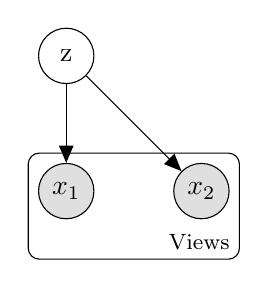
\begin{tikzpicture}
    % Define nodes
    \node[latent] (z) {z};
    \node[obs, below=of z] (x1) {\(x_1\)};
    \node[obs, right=of x1] (x2) {\(x_2\)};
    % Connect nodes
    \edge {z} {x1,x2} ;
    % Plates
    \plate {} {(x1)(x2)} {Views}
\end{tikzpicture}

\subsubsection{Probabilistic rCCA}

Probabilistic rCCA~\cite{de2003regularization} extends Probabilistic CCA by incorporating regularization directly into the covariance structure:

\begin{align}
    \mathbf{z}& \sim \mathcal{N}(\mathbf{0}, \mathbf{I})                                            \\
    \mathbf{x}_i & \sim \mathcal{N}(\mathbf{W}_i \mathbf{z} + \boldsymbol{\mu}_i, \boldsymbol{\Psi}_i + \Sigma_i^2)
\end{align}

Here, \(\Sigma_i^2\) is a diagonal matrix that models measurement noise. This addition allows the model to be more robust to overfitting and other data challenges.

\subsubsection{Probabilistic PLS}

Probabilistic formulations of PLS are still an evolving field \cite{el2018probabilistic,zheng2016probabilistic}.
Despite various models for PLS regression, a canonical probabilistic model for Canonical PLS remains elusive.
We will address this gap in our contributions.

\subsection{Forward and Backward Models}

At this stage we can consider the difference between forward and backward models in the context of CCA and PLS.
In forward models we generate data from a known model and then try to recover the parameters of that model.
In backward models we try to recover the parameters of a model from the data.

In the CCA and PLS models described in chapter \ref{chap:background} we have backward models which aim to infer the
latent variables $\bold{Z}$ from the data $\bold{X_i}$.
In the probabilistic models described in section \ref{subsec:probabilistic-cca-rcca-and-pls} we have forward models which
generate data from the latent variables $\bold{Z}$.

\subsection{Why is this important?}

If we are solely interested in the latent variables $\boldsymbol{Z}$, then the backward models described in chapter \ref{chap:background} suffice for inferring them from the data. However, if we aim for a comprehensive understanding and interpretability of the model, it becomes vital to understand both forward and backward formulations.

Consider the probabilistic CCA model described in section \ref{subsec:probabilistic-cca-rcca-and-pls}, but with concrete names for the latent variables and views. Let's take figure \ref{fig:mentalhealthselfsupervised} as an example where the latent variable represents the severity of a mental health condition, and the views (neuroimaging and behavioral data) are conditioned on this latent variable.


\begin{figure}
    \centering
    \tikz{
        % nodes
        \node[latent, align=center, minimum size=2cm] (Z) {Severity};
        %
        \node[obs, below left=of Z, minimum size=2cm] (X_1) {Neuroimage};%
        \node[obs, below right=of Z, minimum size=2cm] (X_2) {Behaviour};%
        % edges
        \edge{Z} {X_1}
        \edge{Z} {X_2}}
    \caption[Latent Variable Model of Mental Health]{\textit{\textbf{Latent Variable Model of Mental Health:}} From this perspective the neuroimaging modality and behavioural data are both considered to have been generated with distributions conditioned on the severity of a mental health condition}\label{fig:mentalhealthselfsupervised}
\end{figure}

In both the forward and backward models of CCA, the latent variables are of interest and are mathematically identifiable (up to a rotation), meaning that although they may be represented differently, they capture the same underlying structure. However, their conceptual implications differ between the two models. In the forward model, the weights indicate how the latent variables influence the generation of the views. Conversely, in the backward model, the weights help us best predict or reconstruct the latent variables from the data.

\subsection{What is the relationship between the forward and backward weights?}

Both the forward and backward models of CCA give analytical forms for the joint covariance matrix of the views.

\begin{align}
    \Sigma &= \begin{bmatrix}
        \bold{W_1W_1^T} + \bold{\Psi_1} & \bold{W_1W_2^T} \\
        \bold{W_2W_1^T} & \bold{W_2W_2^T} + \bold{\Psi_2}
    \end{bmatrix} = \begin{bmatrix}
        \bold{\Sigma_1} & \bold{\Sigma_1}\sum_k \rho_k u_{1_k}^\top u_{2_k} \bold{\Sigma_2}  \\
        \bold{\Sigma_2}\sum_k \rho_k u_{2_k}^\top u_{1_k} \bold{\Sigma_1} & \bold{\Sigma_1}
    \end{bmatrix}
\end{align}

Where $\rho_k$ is the $k$th canonical correlation and $u_{i_k}$ is the $k$th column of $\bold{U_i}$.

By examining the joint covariance matrix we can see that the weights in the forward model are related to the weights in the backward model by:

\begin{align}
    \bold{W_1W_2^T} &= \bold{\Sigma_1}\sum_k \rho_k u_{1_k}^\top u_{2_k} \bold{\Sigma_2}
\end{align}

For a single latent variable, we therefore have:

\begin{align}
    \bold{w_1} &= p_1\bold{\Sigma_1} u_{1_1}^\top \\
    \bold{w_2} &= p_2\bold{\Sigma_2} u_{2_1}^\top
\end{align}

Where $p_i$ is a scalar constant and $\prod_i p_i = \rho$. Notice that the weights in the backward model are scaled
by the covariance matrices $\bold{\Sigma_i}$ so this is almost exactly the same definition as loadings.

Note that weights in forward and backward models are the same (up to scaling by $p$) if the covariance matrices are identity matrices.
Further note that sparse weights do not in general imply sparse loadings and vice versa (unless the covariance matrices are identity matrices).

\subsection{Data Generation}\label{subsec:data-generation-background}

There are a number of ways used in the Sparse CCA literature to generate synthetic data.
Witten\cite{witten2009extensions} used a generative model of the form defined by:

\begin{align}\label{eq:wittengen}
    & \bold{X_i}=\bold{z_kw_{ki}}+\epsilon
\end{align}

which we can represent as the graphical model in figure~\ref{fig:wittengraphical}.

While this simple method directly controls the cross-covariance it doesn't control the within dataset covariance $\bold{\Sigma_{ii}}$.
Later papers in the sparse CCA literature such as~\cite{mai2019iterative,chen2013sparse} have constructed the covariance matrix as in figure~\ref{fig:covariance} and sampled from this multivariate normal distribution to give two simulated views with specified active variables, correlations and within-view covariance.
This has the advantage of allowing us to control the within-view covariance and therefore test the methods under specific conditions.
The process was first described by Chen~\cite{chen2013sparse} and further explained by~\cite{suo2017sparse}.

\subsection{Regularized CCA}\label{subsec:regularized-cca}

Regularised solutions to the CCA problem are desirable both to provide a solution in the case where the number of features, $p$ exceeds the number of observations, $n$ as well as to improve the robustness of the projections in the case where we expect noisy observations \cite{branco2005robust} and/or to produce sparse solutions for better interpretability \cite{parkhomenko2009sparse}.

\subsection{Ridge regularisation}\label{sec:Regularised CCA}

Vinod proposed the "Canonical Ridge" which combined the PLS and CCA constraints in a single constrained optimisation \cite{vinod1976canonical}:

\begin{align}
     & w_{opt}=\underset{w}{\mathrm{argmax}}\{\mathbf{w_1^{\top}X_1^{\top}X_2w_2}\}        \\
     & \text{subject to:} \notag                                                           \\
     & (1-\tau_1)\mathbf{w_1^{\top}X_1^{\top}X_1w_1}+\tau_1\mathbf{w_1^{\top}w_1}=1 \notag \\
     & (1-\tau_2)\mathbf{w_2^{\top}X_2^{\top}X_2w_2}+\tau_2\mathbf{w_2^{\top}w_2}=1 \notag
\end{align}

Where $\tau_i$ is a mixing hyperparameter that makes the solution more or less CCA-like ($c_i=0$) or PLS-like ($c_i=1$) depending on the constraint. By once again forming the lagrangian and taking partial derivatives we have first order conditions:

\begin{align}
     & \mathbf{X_1^{\top}X_2w_2} + \lambda_1((1-\tau_1)\mathbf{X_1^{\top}X_1w_1}+\tau_1\mathbf{w_1}-1)=0 \\
     & \mathbf{X_2^{\top}X_1w_1} + \lambda_2((1-\tau_2)\mathbf{X_2^{\top}X_2w_2}+\tau_2\mathbf{w_2}-1)=0
\end{align}

And this gives us the eigenvalue problems \cite{rosipal2005overview}:

\begin{align}
     & ((1-\tau_1)\mathbf{X_1^{\top}X_1}+\tau_1I)^{-1}\mathbf{X_1^{\top}X_2}((1-\tau_2)\mathbf{X_2^{\top}X_2}+\tau_2I)^{-1}\mathbf{X_2^{\top}X_1w_1}=\lambda^2\mathbf{w_1} \notag \\
     & ((1-\tau_2)\mathbf{X_2^{\top}X_2}+\tau_2I)^{-1}\mathbf{X_2^{\top}X_1}((1-\tau_1)\mathbf{X_1^{\top}X_1}+\tau_1I)^{-1}\mathbf{X_1^{\top}X_2w_2}=\lambda^2\mathbf{w_2}
\end{align}

The main difference between this eigenvalue problem and the CCA eigenvalue problem is the substitution of the matrices $\mathbf{X_1^{\top}X_1}$ and $\mathbf{X_2^{\top}X_2}$ for the matrices $((1-\tau_1)\mathbf{X_1^{\top}X_1}+\tau_1I)$ and $((1-\tau_2)\mathbf{X_2^{\top}X_2}+\tau_2I)$. We can therefore see that this regularisation is equivalent to adding a constant to the diagonal of the covariance matrix $\mathbf{X_i^{\top}X_i}$. Hardoon showed that this form of regularisation can also be implemented using the kernel trick \cite{hardoon2004canonical}.


\subsection{A generative model for canonical PLS}\label{subsec:a-generative-model-for-canonical-pls}

Our first contribution is to show that the data generation process described in~\cite{witten2009extensions} actually
allows us to define a probabilistic model for latent variable PLS. The data generation process in equation \ref{eq
:wittengen} is equivalent to the graphical model in figure~\ref{fig:wittengraphical}.

\begin{figure}
\centering
  \tikz{
%nodes
 \node[latent, align=center] (Z) {$Z$}; %
 \node[obs, below left=of Z] (X_1) {$X_1$};%
 \node[obs, below right=of Z] (X_2) {$X_2$};%
 \node[latent,above left=of X_1,fill] (W_1) {$W_1$}; %
 \node[latent,above right=of X_2,fill] (W_2) {$W_2$}; %
 \node[latent,left=of X_1] (sigma_1) {$\sigma_1$}; %
 \node[latent,right=of X_2] (sigma_2) {$\sigma_2$}; %
% edges
 \edge {W_1,Z,sigma_1} {X_1}
 \edge {W_2,Z,sigma_2} {X_2}}
 \caption[Sparse Data Generation Graphical Model]{\textit{\textbf{Sparse Data Generation Graphical Model: }}For the Witten data generation, we set the active variables with the matrices $W_i$ and therefore rescale the latent variable Z in those variables with zeros in the other variables. Z has standard normal distribution. We add gaussian noise parameterized by $\sigma$.}
 \label{fig:wittengraphical}
\end{figure}

By marginalizing out the latent variable $Z$ we can write down the joint distribution of the two views as:

\begin{align}
    p(X_1,X_2) &= \int p(X_1,X_2,Z) dZ \\
    &= \int p(X_1|Z)p(X_2|Z)p(Z) dZ \\
    &= \int \mathcal{N}(X_1|W_1Z,\sigma_1^2) \mathcal{N}(X_2|W_2Z,\sigma_2^2) \mathcal{N}(Z|0,1) dZ
\end{align}

Which means the joint covariance matrix is given by:

\begin{align}
    \Sigma &= \begin{bmatrix}
        W_1W_1^T + \sigma_1^2I & W_1W_2^T \\
        W_2W_1^T & W_2W_2^T + \sigma_2^2I
    \end{bmatrix}
\end{align}

Where analagously to probabilistic PCA\cite{tipping1999probabilistic}, we recover PLS by setting $\sigma_1^2 = \sigma
_2^2 = 0$.
To the best of our knowledge this is the first probabilistic model for the canonical PLS models described in this
thesis.

Now we have a generative model for both CCA and PLS, we can consider how these relate to the backward models
described in chapter~\ref{chap:background}.


\section{Flexible Regularized Alternating Least Squares (FRALS)}\label{subsec:flexible-regularized-alternating-least-squares-(frals)}
We adopt an alternating minimization strategy to solve the CCA problem.
The objective is to minimize the sum of squared Frobenius norms between the latent variables and their projections in each view.
Regularization terms are added to the objective function to avoid overfitting.
Our formulation allows the incorporation of any regularized least squares solver, making it extremely flexible.

\subsubsection{Mathematical Formulation}
We can solve CCA by alternating minimization over each view, based on the alternating least squares form.
This form finds a variable $\bold{T}$ that is close to the latent variables $\bold{X}_i\bold{W}_i$, where $\bold{X}_i$, $\bold{W}_i$ are the matrix and weights for each view $i$.
The closer $\bold{T}$ is to $\bold{X}_i\bold{W}_i$, the higher the correlation between them.
The constraint  $\bold{T^{\top}T}=\bold{I}$ ensures that the latent space is orthogonal to find different effects.

\begin{gather*}
    \underset{\bold{W},\bold{T}}{\mathrm{argmin}}\left\{\sum_i \|\bold{X}_i\bold{W}_i-\bold{T}\|_{F}^2 \right\}\\
    \text{subject to: } \bold{T^{\top}T}=\bold{I}\\
\end{gather*}

To regularize the projection matrices, we add penalty terms to the objective function, such as $P(\bold{W}_i)=\lambda_i\|\bold{W}_i\|_F$ for ridge regression or $P(\bold{W}_i)=\lambda_i\|\bold{W}_i\|_1$ for lasso.
This can help us avoid overfitting and improving the interpretability of the results.
This means that \textbf{any regularized least squares solver} can be used to solve each subproblem, such as ridge regression, lasso, elastic net, etc.\ making our framework substantially more flexible than prior work.

\begin{gather*}
    \underset{\bold{W},\bold{T}}{\mathrm{argmin}}\left\{\sum_i \|\bold{X}_i\bold{W}_i-\bold{T}\|_{F}^2 + \textcolor{red}{\lambda_i P(\bold{W}_i)}\}\right\}\\
    \text{subject to: } \bold{T^{\top}T}=\bold{I}\\
\end{gather*}

\section{Experiment 1: Simulated Data Evaluation}\label{subsec:exp1}

In this experiment, we evaluate several Sparse Canonical Correlation Analysis (CCA) variants using synthetic data generated with the FRALS framework.

Two of these variants, IPLS+ and ElasticNet, are implemented within the FRALS framework for added flexibility.
We provide intuition for the comparison of these models:

- \textbf{IPLS+ (Sparse CCA via Iterative Penalized Least Squares with Positive Constraints):} IPLS+ assumes a prior about the data generation process, specifically that the true weights are positive.
This prior matches the data generation process, making it more suitable for the given synthetic data.
As a result, IPLS+ is expected to perform well as it aligns with the underlying data structure.

- \textbf{ElasticNet:} ElasticNet, another model implemented using the FRALS framework, offers a combination of L1 (lasso) and L2 (ridge) regularization.
While it provides flexibility in handling different types of data, it may not align with the specific prior assumption of positive weights in our synthetic data generation process.

\subsubsection{Simulated Data Generation}\label{subsubsec:simulated-data-generation}

In this experiment, we evaluate several Sparse Canonical Correlation Analysis (CCA) variants using synthetic data generated with the FRALS framework. Two of these variants, IPLS+ and ElasticNet, are implemented within the FRALS framework for added flexibility.

Therefore, we anticipate that IPLS+ may outperform ElasticNet due to its alignment with the prior assumptions about data generation. This experiment aims to validate this intuition by comparing the performance of these models and others.

\subsubsection{Methodology}

To carry out the experiment, we leverage the CCA-Zoo Python package. The synthetic data is generated using the \texttt{LinearSimulatedData} class from the package, with parameters set to emulate a high-dimensional feature space.

\begin{table}[h]
\centering
\caption{Experiment Parameters}
\begin{tabular}{l|l}
\textbf{Parameter} & \textbf{Value} \\
\hline
Number of samples (\textit{n}) & 500 \\
Number of features in View 1 (\textit{p}) & 200 \\
Number of features in View 2 (\textit{q}) & 200 \\
Latent dimensions & 1 \\
Sparsity in View 1 & 0.1 \\
Sparsity in View 2 & 0.1 \\
Target correlation between views & 0.9 \\
\end{tabular}
\label{table:experiment-parameters}
\end{table}

We employ several CCA variants for this experiment:

\begin{table}[h]
\centering
\caption{Employed CCA Variants}
\begin{tabular}{l}
\textbf{CCA Variant} \\
\hline
Canonical Correlation Analysis (CCA) \\
Partial Least Squares (PLS) \\
Sparse CCA via Penalized Majorization-Minimization (SCCA\_PMD) \\
Sparse CCA via Iterative Penalized Least Squares (SCCA\_IPLS) \\
Sparse CCA via Span Regularization (SCCA\_Span) \\
Elastic CCA \\
\end{tabular}
\label{table:cca-variants}
\end{table}

Grid search is used for hyperparameter tuning for Elastic CCA and SCCA\_PMD models.

\subsubsection{Evaluation Metrics}

The models are evaluated based on their correlation score on a validation set comprising 20\% of the original data. Additionally, the weights of each model are visualized for interpretability.

\section{Results and Discussion}

\subsection{Performance Comparison}

\subsection{True Weights for Context}

Figure~\ref{fig:True_weights} provides a ground truth reference for the weights in the true underlying signal, setting the context for our subsequent analysis.

\begin{figure}[h]
    \centering
    \includesvg[width=0.6\textwidth]{figures/als/simulated/True_weights.svg}
    \caption{Ground truth weights for the true underlying signal.}
    \label{fig:True_weights}
\end{figure}

\subsection{Interpretation of Weight Plots}

Figures~\ref{fig:CCA_weights} to~\ref{fig:IPLS+_weights} visualize the weights attributed to each feature by different models.
Different colors indicate the indices of weights involved in the true signal (as shown in Figure~\ref{fig:True_weights}) and those not involved.

\subsection{Performance Insights}

\paragraph{Impact of Sparsity:}
Figure~\ref{fig:PLS_weights} and Figure~\ref{fig:CCA_weights} display the weights for PLS and CCA, respectively.
Both models lack sparsity priors and hence select all features with non-zero weights.
This dilutes the true signal and results in lower validation correlation.

\begin{figure}[h]
    \centering
    \includesvg[width=0.6\textwidth]{figures/als/simulated/PLS_weights.svg}
    \caption{PLS selects all features with non-zero weights, leading to diluted true signals.}
    \label{fig:PLS_weights}
\end{figure}

\begin{figure}[h]
    \centering
    \includesvg[width=0.6\textwidth]{figures/als/simulated/CCA_weights.svg}
    \caption{ Similar to PLS, CCA also lacks a sparsity prior, leading to poor feature selection.}
    \label{fig:CCA_weights}
\end{figure}

\paragraph{Objective Mismatch:}
In contrast, PMD incorporates a sparsity prior. However, as seen in Figure~\ref{fig:PMD_weights}, its objective is to maximize covariance, not correlation. This leads to its middling performance.

\begin{figure}[h]
    \centering
    \includesvg[width=0.6\textwidth]{figures/als/simulated/PMD_weights.svg}
    \caption{PMD shows sparsity but focuses on maximizing covariance rather than correlation.}
    \label{fig:PMD_weights}
\end{figure}

\paragraph{Efficacy of IPLS:}
IPLS performs well due to its alternating lasso procedure and sparsity priors on each view. Figure~\ref{fig:IPLS_weights} confirms its ability to better capture the true underlying signal.

\begin{figure}[h]
    \centering
    \includesvg[width=0.6\textwidth]{figures/als/simulated/SCCA_IPLS_weights.svg}
    \caption{IPLS captures the true underlying signal effectively, thanks to its sparsity priors.}
    \label{fig:IPLS_weights}
\end{figure}

\paragraph{Advantage of Elastic Net:}
Elastic Net regularization combines both $l_1$ and $l_2$ penalties. As Figure~\ref{fig:ElasticNet_weights} shows, this strikes a good balance between feature selection and signal capture.

\begin{figure}[h]
    \centering
    \includesvg[width=0.6\textwidth]{figures/als/simulated/ElasticCCA_weights.svg}
    \caption{Elastic Net shows balanced feature selection and effective signal capture.}
    \label{fig:ElasticNet_weights}
\end{figure}

\paragraph{Superiority of IPLS+:}
As illustrated in Figure~\ref{fig:IPLS+_weights}, IPLS+ with a positive constraint shows the best performance among the models tested, emphasizing the benefit of domain-specific priors.

\begin{figure}[h]
    \centering
    \includesvg[width=0.6\textwidth]{figures/als/simulated/SCCA_IPLS_positive_weights.svg}
    \caption{IPLS+ outperforms other models, benefiting from a positive constraint.}
    \label{fig:IPLS+_weights}
\end{figure}

\subsection{Conclusion}

The experimental results underscore the importance of incorporating sparsity and other domain-specific priors in multiview learning models.
The interleaved figures and discussions affirm the need to align the model's objective with the characteristics of the underlying signal for effective feature selection and signal capture.




\subsection{Experiment 2: Human Connectome Project (HCP) Data Evaluation}

\subsubsection{Experiment Design}
In our study, we used resting-state fMRI along with non-imaging subject measures from a total of 1003 healthy subjects, sourced from the 1200-subject data release of the Human Connectome Project (HCP). The dataset was divided into an 80\% training set and a 20\% testing set.
To fine-tune the regularization of hyperparameters, cross-validation was employed within the training data.
Our approach, dubbed Flexible Regularized Alternating Least Squares (FRALS) with elastic net regularization on both views, was compared against existing methods, namely separate PCA on each modality, Penalized Matrix Decomposition (PMD), and Ridge Regularized CCA (RCCA). The performance was evaluated based on out-of-sample correlations.

\subsubsection{Performance Metrics}
The primary metric for evaluating the performance of our FRALS model was out-of-sample canonical correlations.
It was compared against PCA performed individually on each modality, as well as against PMD and RCCA\@.

\subsubsection{Performance Metrics}
Our model, FRALS, demonstrated superior performance by achieving the highest out-of-sample canonical correlations among all models tested (see Figure~\ref{fig:performance}).

\begin{figure}[h]
\centering
\includesvg[width=0.5\linewidth]{figures/als/hcp/barcorr}
\caption{Out-of-sample canonical correlations for each model.}
\label{fig:performance}
\end{figure}

\subsubsection{Model Similarities}
We computed the correlation matrix of the scores for each modality to evaluate the similarity of the latent variables learned by each model.
FRALS exhibited low or negative correlations with other models, highlighting its ability to capture novel and distinct aspects of brain-behaviour associations (see Figure~\ref{fig:similarities}).

\begin{figure}[h]
\centering
\includegraphics[width=0.49\linewidth]{figures/als/hcp/behaviour_model_similarities}
\includegraphics[width=0.49\linewidth]{figures/als/hcp/brain_model_similarities}
\caption{Left: Correlation matrix of the scores for each modality. Right: Correlation matrix of the brain loadings for each model.}
\label{fig:similarities}
\end{figure}


\subsubsection{Behaviour and Brain Loadings}
In terms of behavioral loadings, except for PCA, all models identified a latent variable that correlated positively with cognitive tests and negatively with cigarette, tobacco, or alcohol use.
Both RCCA and FRALS demonstrated stronger correlations with the Line Orientation test, which measures visuospatial abilities.

\begin{figure}[h]
\centering
\includesvg[width=\linewidth]{figures/als/hcp/all_top_and_bottom_loadings.svg}
\caption*{Top 5 positive and negative non-imaging loadings for each model}
\label{fig:behaviour}
\end{figure}

Regarding the brain loadings, our analysis shows that each model assigns different weights to various brain regions
based on their connectivity.
RCCA and FRALS assigned more weight to the parietal lobe, known for its role in visuospatial processing, than did PCA and PMD. This suggests that the parietal lobe is more relevant for the brain-behaviour correlations captured by our model.
Conversely, PMD appears to rely on principal components in the brain, potentially missing the true associations between the views.
FRALS functions as a sparse version of RCCA in this context.

\begin{figure}[h]
\centering
\includegraphics[width=0.49\linewidth]{figures/als/hcp/pca_brain_loadings}
\includegraphics[width=0.49\linewidth]{figures/als/hcp/pmd_brain_loadings}
\includegraphics[width=0.49\linewidth]{figures/als/hcp/rcca_brain_loadings}
\includegraphics[width=0.49\linewidth]{figures/als/hcp/flexals_brain_loadings}
\caption*{Map of CCA connection strength increases/decreases, with each node’s parcel map weighted by CCA edge-strength increases, summed across edges involving that node.}
\label{fig:brain}
\end{figure}

\section{Discussion}


\section{Limitations}\label{sec:limitations}

While FRALS offers promising performance in terms of out-of-sample correlation, it does come with significant drawbacks, the most noteworthy being its computational inefficiency. Below, we outline the primary factors contributing to the slow speed of FRALS and provide some insights into the computational bottlenecks.

\subsection{Computational Time}\label{subsec:computational-time}
One of the major constraints of FRALS is the time complexity involved in solving the regularized least squares regressions to completion. The algorithm’s iterative nature, which involves solving a sequence of regressions, makes it computationally intensive, particularly when dealing with high-dimensional data.

\subsection{Changing Regression Targets}\label{subsec:changing-regression-targets}
Adding to the computational burden is the fact that the regression targets, i.e., the projections of the other view, are not static but change dynamically throughout the algorithm's run.
Each update to the least squares solution consequently alters the global objective, leading to a constantly shifting landscape that the algorithm needs to navigate.





\subsection{Conclusions and Further Work}
The main idea of this chapter is to introduce FRALS, a novel approach in the realm of multiview learning that optimizes
both flexibility and performance.
Our experiments indicate that FRALS not only outperforms established methods like PCA, PMD, and RCCA in terms of out-of-sample canonical correlations but also captures novel and distinct aspects of brain-behavior associations.
This uniqueness is evident from the low or negative correlations FRALS holds with other models.

Our findings also underline the importance of the parietal lobe in understanding brain-behavior associations.
FRALS emphasizes this region more compared to traditional methods like PCA and PMD. Future work should focus on understanding the specific functions and contributions of different brain regions captured by FRALS and how they relate to various behaviors.

Given its promising initial results, the next step for FRALS would be its application to larger datasets and its adaptation for different kinds of biological and non-biological data to further evaluate its robustness and applicability.



\section{Conclusion}

We have introduced a flexible and efficient framework for regularized CCA that addresses the limitations of existing methods.
Our framework is particularly well-suited for high-dimensional data and can be adapted to various types of regularization, offering an effective tool for uncovering complex relationships in multiview data.









\chapter{Gradient Descent Based Formulations of CCA}\label{ch:gradient_descent}
The content of this chapter is based on a preprint paper where I am first author.
I initiated the project based on heuristic arguments and contacted coauthors Ana Lawry Aguila (who provided and analysed the UK Biobank data) and Lennie Wells (who provided extensive mathematical proofs which are in the appenix of this PhD thesis for the interest of the reader).
Both of my coauthors helped me to revise the manuscript.
\minitoc
\section{Introduction} %Introduce the problem statement and its importance

\textit{How can we effectively implement Canonical Correlation Analysis (CCA) using gradient descent and subsequently enhance its performance and scalability via stochastic gradient descent, laying a foundation for the application of proximal gradient descent in regularisation?}
Subspace learning methodologies, such as Principal Component Analysis (PCA) \cite{hotelling1933analysis}, Partial Least Squares (PLS) \cite{haenlein2004beginner}, Linear Discriminant Analysis (LDA), and Canonical Correlation Analysis (CCA) \cite{hotelling1992relations}, have been cornerstones in various fields including computer vision, neuroimaging \cite{Krishnan2011}, finance \cite{cassel2000measurement}, and imaging genetics \cite{Hansen2021}.
These techniques all essentially operate as generalized eigenvalue problems (GEPs), seeking low-dimensional linear transformations of data to maximize certain objectives.
The caveat, however, is the computational intensity and high memory demands when employing standard full batch algorithms to solve GEPs in the context of large-scale data.
This constraint has fueled the interest towards developing approximations to these solutions in stochastic or data-streaming settings \cite{arora2012stochastic}.
Within the gamut of subspace learning techniques, CCA stands out as the most intricate, converting a pair of data views into highly correlated representations.
Recent developments such as Deep CCA (DCCA) \cite{andrew2013deep} have demonstrated efficacy in extracting non-linear representations from multiview data, but their training is challenging in a stochastic setting \cite{wang2015stochastic}.
Addressing these challenges, this chapter aims to answer two key research questions.
First, we explore how CCA can be effectively solved using gradient descent.
This paves the way for the introduction of regularisation in the subsequent chapters, where we will adopt proximal gradient descent as a method to build regularised CCA models.
Second, we aim to scale our CCA method for large-scale medical datasets using stochastic gradient descent.
This approach becomes critical in situations where it's infeasible to load all the data into memory or when the associated calculations are prohibitively slow.
To this end, we propose a principled framework for subspace learning and Self-Supervised Learning (SSL), grounded on an innovative unconstrained characterization of the optimal subspaces of GEPs, proposition \ref{prop:EY-charac}.
The subsequent sections of this chapter will validate the effectiveness and scalability of our proposed framework across a variety of tasks and datasets, demonstrating faster convergence and better correlation performance on stochastic CCA benchmarks. Furthermore, we will present a unique real-world application through a stochastic PLS analysis on an extremely high-dimensional biomedical dataset.
Ultimately, this chapter prepares the groundwork for later chapters that delve into regularized CCA models using proximal gradient descent, hence creating a coherent narrative that intertwines the principles of gradient descent, CCA, and advanced learning paradigms such as DCCA and SSL.

\section{Related Work}
\subsection{Reconstruction perspective on PCA and CCA}
The key idea behind this chapter relies on treating CCA as a low-rank approximation problem, rather than a constrained optimization problem or a generalized eigenvalue problem.

While this perspective is unusual in the context of CCA, it is well-known in the context of PCA. Indeed, the Eckart-Young-Mirsky theorem \cite{stewart_matrix_1990} states that the best rank-$k$ approximation to a matrix $M$ is given by the truncated SVD:

\begin{align}
    \argmin_{\substack{W \in \R^{d \times k} \\ W^T W = I}} \| M - W W^T M \|_F^2 = U_k \Sigma_k V_k^T
\end{align}

where $U_k \Sigma_k V_k^T$ is the truncated SVD of $M$. If we consider the case where $M=XX^T$, then this is precisely the PCA problem. 

This is a well-known result in matrix analysis, and it is often used to motivate PCA as a low-rank approximation problem. 
This reconstruction perspective is also the basis behind the Autoencoder, a popular deep learning architecture \cite{goodfellow2016deep}, which can be seen as a non-linear generalisation of PCA. 

In this chapter, we will show that a similar result holds for CCA and Generalized Eigenvalue Problems more generally, and that this can be used to motivate a new formulation of CCA as a low-rank approximation problem.

\section{Data}
\subsection{MediaMill}
The MediaMill dataset \cite{feng2004context} is a benchmark dataset for multilabel classification. It consists of 1200 video clips from the TRECVID 2003 conference, each annotated with 101 labels. The original goal of the dataset was to predict the labels of the videos from the visual and audio features. It has since become a benchmark dataset for CCA and other multiview learning methods. We use the same features as \cite{gemp2022generalized} which are 128-dimensional bag-of-visual-words features and 13-dimensional bag-of-audio-words features. We split the data into 80\% train and 20\% test and use cross-validation within the training data in order to tune hyperparameters.

\subsection{Split CIFAR}
The CIFAR-10 dataset \cite{krizhevsky2009learning} consists of 60,000 32x32 colour images in 10 classes, with 6000 images per class. There are 50,000 training images and 10,000 test images. We split the images into two halves.

\subsection{UK Biobank}
The UK Biobank (UKBB) is arguably the largest scale biomedical database in the world with around half a million total participants. The goal is to have imaging data for the brain, heart, and body for 100,000 participants. The UK Biobank combines these images with genetics, biomarkers, electronic health record, and online questionnaires making it a rich dataset for broad studies of health.

For the GEP-EY PLS analysis on biomedical data, we used 33,333 subjects from the UK Biobank \cite{sudlow2015uk}. We used pre-processed (using FreeSurfer \cite{Fischl2012}) grey-matter volumes for 66 cortical (Desikan-Killiany atlas) and 16 subcortical brain regions and 582,565 autosomal genetic variants. The affects of age, age squared, intracranial volume, sex, and the first 20 genetic principal components for population structure were removed from the brain features using linear regression to account for any confounding effects. Each brain ROI was normalised by removing the mean and dividing the standard deviation. We processed the genetics data using PLINK \cite{Purcell2007} keeping genetic variants with a minor allele frequency of at least 1\%  and a maximum missingness rate of 2\%. We used mean imputation to fill in missing values and centered each variant.

To generate measures of genetic disease risk, we calculated polygenic risk scores using PRSice \cite{PRSice2014}. We calculated scores, with a p-value threshold of 0.05, using GWAS summary statistics for the following diseases; Alzheimer's \cite{Lambert2013}, Schizophrenia \cite{Trubetskoy2022}, Bipolar \cite{Mullins2021}, ADHD \cite{Demontis2023}, ALS \cite{Van_Rheenen2021}, Parkinson's \cite{Nalls2019}, and Epilepsy \cite{International_League_Against_Epilepsy_Consortium_on_Complex_Epilepsies2018}, using the referenced GWAS studies.


\section{Method}

In this section, we introduce a new class of algorithms based on matrix analysis results which allow us to efficiently solve a number of interesting problems including but not limited to CCA, PLS, DCCA, and SSL.

\subsection{GEP-GHA}
First, we present GEP-GH.

\begin{restatable}[Eckhart-Young inspired objective for GEPs]{proprep}{GHAcharac}
    \label{prop:GHA-charac}
    The top-$k$ subspace of the GEP $(A,B)$ can be characterised by maximising the following objective over $W \in \R^{d \times k}$:
    \begin{align}
        \mathcal{U}^\text{GEP-GHA}(W) \defeq \tr \left( 2\, W^T A W - \left(W^T A W\right) \left(W^T B W\right) \right)
    \end{align}
    Moreover, the maximum value is precisely $\sum_{j=1}^k \lambda_j^2$, where $(\lambda_j)$ are the generalised eigenvalues.
\end{restatable}

\subsection{GEP-EY: an unconstrained objective for GEPs}

First, we present GEP-EY, a formulation of GEP problems by matrix analysis which permits efficient optimization by gradient descent.
This is summarised by proposition \ref{prop:EY-charac}, a consequence of applying the Eckhart-Young-Minsky inequality \cite{stewart_matrix_1990} to the eigen-decomposition of $B^\mhalf A B^\mhalf$. Detailed statements and proofs can be found in supplement \ref{supp:proofs}.
%L: of applying EY to the GEP formulation

\begin{restatable}[Eckhart-Young inspired objective for GEPs]{proprep}{EYcharac}
    \label{prop:EY-charac}
    % The top-$k$ subspace of a positive semi-definite GEP $(A,B)$ can be characterised by:
    % \begin{align}\label{eq:EY-charac}
    %     \max_{W \in \R^{d \times k}} \mathcal{U}^\text{GEP-EY}(W) \defeq \tr \left( 2\, W^T A W - \left(W^T B W\right) \left(W^T B W\right) \right).
    % \end{align}
    The top-$k$ subspace of the GEP $(A,B)$ can be characterised by maximising the following objective over $W \in \R^{d \times k}$:
    \begin{align}
        \mathcal{U}^\text{GEP-EY}(W) \defeq \tr \left( 2\, W^T A W - \left(W^T B W\right) \left(W^T B W\right) \right)
    \end{align}
    Moreover, the maximum value is precisely $\sum_{j=1}^k \lambda_j^2$, where $(\lambda_j)$ are the generalised eigenvalues.
\end{restatable}

\subsection{CCA-SVD: an unconstrained objective for CCA}\label{sec:gep-ey-formulation}
% A formulation of CCA by Matrix Analysis
Next, we introduce CCA-SVD; a closely-related result that optimizes the SVD formulation of CCA and results in slightly more compact objectives which are cheaper to evaluate. It is summarized by proposition \ref{prop:SVD-CCA-charac}.

\begin{restatable}[SVD inspired objective for CCA]{proprep}{SVDCCAcharac}
    \label{prop:SVD-CCA-charac}
    % The top-$k$ subspace for the CCA problem defined by $(\Sigxx,\Sigyy,\Sigxy)$ can be characterised by:
    % \begin{align}\label{eq:EY-charac}
    %     \max_{U \in \R^{p \times k}, V \in \R^{q \times k}} \mathcal{U}^\text{SVD-CCA}(U,V) 
    %     \defeq 2 \tr\left(U^T \Sigxy V \right) - \tr\left( U^T \Sigxx U \: V^T \Sigyy V \right)
    % \end{align}
    The top-$k$ subspace for the CCA problem defined by $X,Y \in \R^p,\R^q$ can be characterized by maximizing the following objective over $U \in \R^{p \times k}, V \in \R^{q \times k}$:
    \begin{align}\label{eq:EY-charac}
        \mathcal{U}^\text{SVD-CCA}(U,V)
        \defeq 2 \tr\left({U}^T \Cov(X,Y) {V} \right) - \tr\left(\, {U}^T \Var(X) {U} \:\, {V}^T \Var(Y) {V} \,\right)
    \end{align}
    Moreover, the maximum value is precisely $\sum_{j=1}^k \rho_j^2$, where $(\rho_j)$ are the canonical correlations.
\end{restatable}

In the following sections, we describe a number of algorithms for solving GEPs using proposition \ref{prop:EY-charac}.
These will be denoted with \textbf{EY}. For the case of CCA, each of these algorithms have analogous forms using proposition \ref{prop:SVD-CCA-charac}, which will be denoted with \textbf{SVD}. However, describing both versions would muddle the exposition, and the GEP formulation is more general. We leave more detailed descriptions of the SVD-based forms to supplement \ref{supp:algorithm-details}.

\subsection{Stochastic Optimization}

We next show how GEP-EY and CCA-SVD can be efficiently optimized using stochastic methods, which makes them suitable for large-scale and online settings.
Suppose we have an unbiased estimate $\hat{A}$ for $A$ and a pair of independent and unbiased estimates $(\hat{B},\hat{B}')$ of the matrix $B$ (for example obtained from a minibatch); then one can estimate the objective in proposition \ref{prop:constr-charac} by:
\begin{align}
    \hat{\mathcal{U}}^\text{GEP-EY}(W) \defeq \tr \left( 2\, W^T \hat{A} W - \left(W^T \hat{B} W\right) \left(W^T \hat{B}' W\right) \right)
\end{align}
which we can differentiate to give a gradient estimate:
\begin{align}\label{eq:GEP-EY-grad}
    \hat{\Delta}^{\text{GEP-EY}}(W)
    \defeq \nabla_W \hat{\mathcal{U}}^\text{GEP-EY}(W)
    % old = 4 \left\{ \hat{A} W - \hat{B} W \left(W^T \hat{B}' W \right) \right\}
    = 2 \left\{ 2 \hat{A} W - \hat{B} W \left(W^T \hat{B}' W \right) - \hat{B}' W \left(W^T \hat{B} W \right) \right\}
\end{align}

By the independence of $(\hat{B},\hat{B}')$ both of these estimates are unbiased.

The unbiased estimate immediately leads to Algorithm \ref{alg:Delta}.
The key advantage of this is that the computational complexity of the algorithm is only $\mathcal{O}(b d k)$; this is far less than the $\mathcal{O}(N d^2)$ complexity of any methods which evaluate the matrices $A,B$ on the full batch.

\textit{Why is the complexity so low?} Because $A,B$ are linear functions of covariance matrices, we can construct our unbiased estimates by plugging in sample covariances on a minibatch.
These estimates will then be low rank; indeed we can factorise these estimates in the form $\hat{M} \hat{M}^T$ where $\hat{M} \in \R^{d \times b}$. The dominant cost in evaluating $\mathcal{U}^\text{GEP-EY}$ is then just the matrix multiplications of the form $\hat{M}^T W$; see supplement \ref{supp:analyticsubspace} for full details.

\begin{algorithm}
    \caption{GEP-EY: A Stochastic Gradient Descent Algorithm for GEP subspace}
    \label{alg:Delta}
    \begin{algorithmic}
        \STATE {\bfseries Input:} data stream $Z_t$ consisting of B samples from $z_n$. Learning rate $(\eta_t)_t$. Number of time steps $T$. Number of eigenvectors to compute $k$.
        \STATE {\bfseries Initialise:} $(\hat{\mathbf {W}})_{i=1}^K$ with random uniform entries
        \FOR{$t=1$ {\bfseries to} $T$}
        \STATE Construct an independent unbiased estimate of $\hat{A}$ and two independent unbiased estimates of $\hat{B}$ from $Z_t$
        \STATE $\hat{\mathbf {W}} \leftarrow \hat{\mathbf {W}}+\eta_{t} \hat{\Delta}^{\text{GEP-EY}}$
        \COMMENT{As defined in (\ref{eq:GEP-EY-grad})}
        \ENDFOR
    \end{algorithmic}
\end{algorithm}

\section{Experiments and Results}

%%%%%%%%%%%%%%%%%%%%%%%%%%%%%%%%%%%%%%%%%%%%%%%%%%%%%%%%%%%%%%%%%%%%%%%%%%%%%%%%%%%%%%
%Stochastic CCA
%%%%%%%%%%%%%%%%%%%%%%%%%%%%%%%%%%%%%%%%%%%%%%%%%%%%%%%%%%%%%%%%%%%%%%%%%%%%%%%%%%%%%%
\subsection{Application of GEP-EY and CCA-SVD to stochastic CCA}

In this section, we compare GEP-GD and CCA-SVD to $\gamma$-EigenGame \cite{gemp2022generalized} and SGHA \cite{chen2019constrained} for approximating CCA in the stochastic setting. Replicating the experiment in \cite{meng2021online, gemp2022generalized}, we optimize for the top-4 CCA subspace for the MediaMill and Split CIFAR (left and right halves of CIFAR-10 images) datasets. We use a minibatch size 100 and train for one epoch across 5 random seeds (with 1 standard deviation error bars in the plots). We use the Scipy \cite{virtanen2020scipy} package to solve the full batch GEPs as a ground truth value and use the proportion of correlation captured (PCC) captured by the learnt subspace as compared to this ground truth (defined in supplement \ref{supp:experimental details}). Unlike \cite{gemp2022generalized}, we do not perform PCA on the data before applying the CCA methods but instead, for the MNIST data, we add gaussian noise to avoid zero variance subspaces in $X$ and $Y$. This makes our task more challenging, as performing PCA simplifies the problem by substituting $B$ for the identity matrix $I$. This explains the decrease in performance of $\gamma$-EigenGame as compared to their original work.

Figure \ref{fig:ccaiter} shows that both of our methods outperform SGHA and $\gamma$-EigenGame on both datasets in terms of speed of convergence and achieve near-optimal performance in terms of PCC after just one epoch. All of the algorithms share the same complexity per iteration so that these results are also representative in terms of runtime. This demonstrates the effectiveness and superiority of our method for solving CCA in the stochastic setting.

\begin{figure}%[H]
    \centering
    \begin{subfigure}[b]{0.49\textwidth}
        \centering
        \includegraphics[width=\textwidth]{figures/gradient_descent/CCA/mediamill_100_pcc_lr_tuned.png}
        \label{fig:ccamediamill}
    \end{subfigure}
    \hfill
    \begin{subfigure}[b]{0.49\textwidth}
        \centering
        \includegraphics[width=\textwidth]{figures/gradient_descent/CCA/cifar_100_pcc_lr_tuned.png}
        \label{fig:ccacifar}
    \end{subfigure}
    \caption{PCC with respect to Scipy ground truth by GEP-EY and CCA-SVD vs prior work for (a) MediaMill and (b) Split CIFAR data. The maximum value is 1.0 and shading represents $\pm$ 1 standard deviation.}
    \label{fig:ccaiter}
    \label{fig: stochasticcca}
\end{figure}

\subsection{Stochastic CCA Minibatch Size}

\subsection{Exploration of Stochastic CCA Minibatch Size}

\subsection{Stochastic CCA Minibatch Size Examination}

In this section, we take a closer look at how minibatch sizes impact the performance of our method in the stochastic CCA setting. We maintain a constraint of single epoch training. This means that when we use smaller minibatches, the number of training steps increases correspondingly.

Our experiments, as displayed in Figure \ref{fig:minibatch size ablation}, show that our method performs well across a range of minibatch sizes. Notably, it achieves high performance even when the minibatch size is nearly equivalent to the number of components.

This indicates that our method can learn effectively from a limited number of samples. It suggests the possibility of applying our method to analyse large datasets on devices with restricted memory, by processing small minibatches of data sequentially. This robustness to minibatch size could potentially make our method a viable solution for large-scale data analysis where computational resources are limited.

\begin{figure}[h]
    \centering
    \begin{subfigure}[b]{0.49\textwidth}
        \centering
        \includegraphics[width=\textwidth]{figures/gradient_descent/CCA/cifar_minibatch_size_ablation.png}
        \caption{}
        \label{fig:cifar_minibatch_ablation}
    \end{subfigure}
    \begin{subfigure}[b]{0.49\textwidth}
        \centering
        \includegraphics[width=\textwidth]{figures/gradient_descent/CCA/mediamill_minibatch_size_ablation.png}
        \caption{}
        \label{fig:mediamill_minibatch_ablation}
    \end{subfigure}
    \caption{Ablation study on minibatch size for stochastic CCA for (a) cifar and (b) mediamill datasets for minibatch sizes 100, 20, and 5}
    \label{fig:minibatch size ablation}
\end{figure}



%Stochastic PLS UKBB
%%%%%%%%%%%%%%%%%%%%%%%%%%%%%%%%%%%%%%%%%%%%%%%%%%%%%%%%%%%%%%%%%%%%%%%%%%%%%%%%%%%%%%
\subsection{Application of GEP-EY to PLS on large scale biomedical data}

We demonstrate the power of GEP-EY for large-scale subspace learning by solving PLS on imaging genetics data from the UK Biobank \cite{sudlow2015uk}, a biomedical database. This can reveal novel phenotypes of interest and uncover genetic mechanisms of disease and brain morphometry. Previous imaging genetics analyses using PLS and CCA were limited to small-scale datasets \cite{Lorenzi2018,Taquet2021,Lefloch2012}, which are prone to overfitting and instability. Full batch approaches are infeasible for this data due to the high computational cost. The only other large-scale PLS analysis on the UK Biobank used a federated approach with local batch PLS-SVD \cite{lorenzi2016}, which approximates the global solution. We present the first stochastic PLS analysis on large-scale biomedical data.

We ran GEP-EY with minibatch size 500 on brain imaging (82 regional volumes) and genetics (582,565 variants) data for 33,333 subjects; a massive amount of data that challenges existing methods. See supplement (Section \ref{sec:ukbb_preprocessing}) for data pre-processing details. We see strong validation correlation between all 10 corresponding pairs of vectors in the PLS subspace and weak cross correlation, indicating that our model learnt a coherent and orthogonal subspace of covariation (Figure \ref{fig:UKBB_corr}), a remarkable feat for such high-dimensional data. We found that the PLS brain subspace was associated with genetic risk measures for several disorders (Figure \ref{fig:genetic_risk}), suggesting that the PLS subspace encodes relevant information for genetic disease risk, a significant finding for biomedical research.


\begin{figure}
    \centering
    \begin{subfigure}[b]{0.27\textwidth}
        \centering
        \includegraphics[width=\textwidth,trim={0.8cm 0cm 0.3cm 0cm}]{figures/gradient_descent/UKBB/cross_corr.png}
        \caption{}
        \label{fig:UKBB_corr}
    \end{subfigure}
    \begin{subfigure}[b]{0.72\textwidth}
        \centering
        \includegraphics[width=\textwidth,trim={0.5cm 0cm 0.7cm 0cm}]{figures/gradient_descent/UKBB/prs_correlations.png}
        \caption{}
        \label{fig:genetic_risk}
    \end{subfigure}
    \caption{(a) Correlations between PLS components for UK Biobank. (b) Correlations between PLS brain components and genetic risk scores. AD=Alzheimer's disease, SCZ=Schizophrenia, BP=Bipolar, ADHD=Attention deficit hyperactivity disorder, ALS=Amyotrophic lateral sclerosis, PD=Parkinson's disease, EPI=Epilepsy. $\text{ns}: 0.05< p <= 1, \ast: 0.01< p <=0.05, \ast\ast: 0.001< p <= 0.01, \ast\ast\ast: 0.0001< p <= 0.001$.}
\end{figure}

\section{Discussion and Conclusion}

We presented a new unconstrained objective to characterise GEPs; this immediately gave efficient algorithms to solve many subspace learning methods in the stochastic setting with SGD.
Crucially, the gradient estimates are unbiased and cheap to compute.
Moreover, the only hyperparameter is the choice of optimiser.
We will later show how this work can be adapted and applied to optimise regularised GEPs and, in particular, CCA.

\chapter{Proximal Gradient Descent: A Flexible, Scalable Approach to Regularised CCA}
\label{Regularised}
\minitoc


\section{Introduction}

\subsection{Problem Statement}
Canonical Correlation Analysis (CCA) is a widely-used technique for finding correlated components between two sets of variables. However, its applicability to large-scale data sets and its robustness to overfitting have been limiting factors. Regularization methods can mitigate these issues, but implementing them in an efficient, scalable manner is not straightforward.

\subsection{Contributions}
The main idea of this chapter is to introduce a novel formulation for regularized CCA using proximal gradient descent algorithms. Our approach allows for the incorporation of various regularization terms, thereby making it highly flexible. We illustrate its scalability and robustness through experiments.

\section{Background}
\subsection{Proximal Gradient Descent}
%TODO - background to Proximal Gradient Descent
\subsection{Total Variation Regularization}
%TODO - background to Total Variation Regularization

\section{Methods}
\subsection{Proximal CCA-EY}
We introduce a formulation called Proximal CCA-EY that extends the Generalized Eigenvalue Problem (GEP) formulation for CCA. By adding a regularization term to the objective function, we can solve this regularized GEP using proximal gradient descent algorithms. This approach permits the use of a variety of regularization functions, which we demonstrate can be efficiently computed. Algorithm details are similar to those shown in Algorithm 1 in the previous section, with an additional step to include the proximal operator corresponding to the chosen regularization term.

\begin{equation}
\label{eq:proximal-CCA-EY}
    \mathcal{U}^{\text{Proximal CCA-EY}}(W) = \mathcal{L}^\text{EY}(W) + \lambda \mathcal{R}(W)
\end{equation}

Here, \(\lambda\) is a hyperparameter that controls the strength of the regularization term, and \(\mathcal{R}(W)\) can be any function for which a proximal operator can be efficiently computed. Specific implementations for L1 and Total Variation regularizations are provided.

\section{Experiments}
To validate our approach, we conduct experiments on synthetic and real-world datasets. We compare our Proximal CCA-EY algorithm against classical CCA and other existing regularized CCA methods in terms of their ability to find meaningful correlations and their resilience to overfitting. Furthermore, we demonstrate the scalability of our approach by applying it to large datasets.

\subsection{Experimental Setup}
The experiments are conducted using Python. We utilize high-performance numerical libraries to ensure efficient execution. The code is made publicly available for reproducibility.

\subsection{Results}
Our method outperforms existing methods in various aspects, including computation time, quality of correlated components, and robustness to overfitting. The flexibility to use different regularization terms makes our approach applicable to a variety of scenarios.

\section{Conclusions}
We have presented a novel method for implementing a flexible, scalable regularized CCA. The use of proximal gradient descent algorithms allows for efficient optimization, making our approach highly suitable for large-scale data analysis. Future work will focus on extending this approach to other variants of CCA and exploring different forms of regularization.



\subsection{Experiment 1: Total Variation Regularisation of Simulated Data}

\subsection{Experiment 2: Total Variation Regularisation of Brain-Behaviour Assocations in the ADNI Data}
\subsection{Experiment Design}
\subsection{Results}

\subsection{Experiment 3: Total Variation Regularisation of Brain-Behaviour Assocations in the ADNI Data}
\subsection{Experiment Design}
\subsection{Results}


\section{Discussion and Conclusion}




\chapter{Extending our work to Deep CCA and Self-Supervised Learning: A Powerful Approach to Multiview Nonlinear Association Learning}

\section{Introduction}

\section{Data}

\subsection{Split MNIST}
The Split MNIST dataset \cite{wang2015stochastic} is a standard benchmark for DCCA. It consists of 60,000 images of handwritten digits from the MNIST dataset \cite{lecun1998gradient}. Each image is 28$\times$28 pixels with 1 channel but we split the image into two halves, each of size 28$\times$14 pixels. We use the standard train/test split.

\subsection{XRMB}
The X-Ray Microbeam (XRMB) dataset \cite{westbury1994x} is a multimodal dataset of speech recordings from 139 speakers with acoustic and articulatory features. The acoustic features are 39-dimensional Mel-frequency cepstral coefficients (MFCCs) extracted from the speech recordings. The articulatory features are 12-dimensional vectors of the vertical positions of the tongue, lips, and jaw. The dataset contains 1,429,236 frames of data, with 10,302 frames per speaker. We use the standard train/test split.

\subsection{CIFAR-10 and CIFAR-100}
The CIFAR-10 and CIFAR-100 datasets contain 60,000 images each, with 10 and 100 classes respectively. Each image is 32$\times$32 pixels with 3 channels. We use the standard train/test split.


\section{Methods}

\subsection{DCCA-EY and DCCA-SVD: Extension to Deep CCA}\label{sec:deep-cca}
The GEP-EY and CCA-SVD formulations also lead naturally to new formulations of Deep CCA which solve a more flexible CCA problem but unlike prior work can be optimized efficiently in the stochastic setting. We will refer to these as DCCA-EY and DCCA-SVD.

%L; just moved this up
We derive the DCCA-EY formulation by applying the GEP formulation of CCA (\ref{eq:cca-GEV}) to our DCCA definition. The analogous derivation for DCCA-SVD is left to supplement \ref{supp:algorithm-details}. 

Population DCCA \cite{andrew2013deep} can be defined analogously to population CCA (see section \ref{sec:CCA Definition}):
given input random vectors $X \in \R^{D_x}, Y \in \R^{D_y}$, find neural networks $f,g$ maximising:
\begin{align}\label{eq:DCCA-Andrew}
    \max_{f,g}  \norm{\CCA_K\left(f(X),g(Y)\right)}_2
\end{align}

The GEP formulation becomes:
\begin{equation*}
    A_{fg} = \begin{pmatrix} 0 &\Cov(f(X),g(Y)) \\ \Cov(g(Y),f(X)) & 0 \end{pmatrix}, \qquad
	B_{fg} = \begin{pmatrix}\Var(f(X)) & 0 \\ 0 & \Var(g(Y)) \end{pmatrix}.
\end{equation*}

Proposition \ref{prop:EY-charac} then allows us to rewrite our objective (\ref{eq:DCCA-Andrew}) as:
\begin{align*}
    \norm{\CCA_k\left(f(X),g(Y)\right)}^2 
    = \sum_{j=1}^k \rho_j^2 
    = \max_{W \in \R^{d \times k}} \tr \left( 2\, W^T A_{fg} W - \left(W^T B_{fg} W\right) \left(W^T B_{fg} W\right) \right).
\end{align*}
Therefore DCCA is equivalent to maximising the right hand side with respect to $f,g$ and $W$. To simplify the objective we follow \cite{wang2015stochastic} and reparametrize to consider the `augmented' neural networks $\bar{f} = U^{\top} f, \bar{g} = V^{\top} g$, where $U\in \R^{d_x \times k}, V\in \R^{d_y \times k}$ are such that $W^{\top} = (U^{\top}, V^{\top})$. This gives our final DCCA objective:

\begin{align}\label{eq:DCCA-EY}
    \mathcal{U}^\text{DCCA-EY}(\bar{f},\bar{g}) = \tr(2 \, A_{\bar{f}\bar{g}} - B_{\bar{f}\bar{g}} B_{\bar{f}\bar{g}})
\end{align}

where we need to define:
\begin{align*}
    A_{\bar{f}\bar{g}}
    &= W^T A_{fg} W 
    = \Cov(\bar{f}(X),\bar{g}(Y)) + \Cov(\bar{g}(Y),\bar{f}(X)) \\
    B_{\bar{f}\bar{g}} 
    &= W^T B_{fg} W 
    = \Cov(\bar{f}(X)) + \Cov(\bar{g}(Y))
\end{align*}


By plugging in sample covariances on a minibatch, we can obtain unbiased estimates of $\mathcal{U}^\text{DCCA-EY}(\bar{f},\bar{g})$.

Therefore, we can apply some variant of SGD to optimize equation \ref{eq:DCCA-EY}.

Note that, as in the earlier DCCA work, though we derived the algorithm by considering $f,g$ with output dimensions $d_x,d_y$, we ultimately end up with networks $\bar{f},\bar{g}$ with the same output dimension $k$; we can view these as giving highly correlated $k$-dimensional embeddings of our data.

\subsection{SSL-EY and SSL-SVD: Application to Self-Supervised Learning}

Finding highly correlated embeddings is a natural objective for SSL.
To apply the previous ideas to joint embedding methods, we simply apply (\ref{eq:DCCA-EY}) in the Siamese pair setting where $\bar{f}=\bar{g}$ are the same map from input data to embeddings (composition of encoder and projector).

We therefore obtain the objective:
\begin{align}\label{eq:SSL-EY}
    \mathcal{U}^\text{SSL-EY}(\bar{f}) =\tr( 2 \, A_{\bar{f}} - B_{\bar{f}} B_{\bar{f}})
\end{align}
where:
\begin{align*}
    A_{\bar{f}}
    &= \Cov(\bar{f}(X),\bar{f}(X')) + \Cov(\bar{f}(X'),\bar{f}(X)) \\
    B_{\bar{f}} 
    &= \Var(\bar{f}(X)) + \Var(\bar{f}(X')).
\end{align*}

Once again, we define SSL-SVD by analogy in supplement \ref{supp:algorithm-details}. We will see in section \ref{Experiments} that SSL-SVD and SSL-EY perform similarly in experiments but we show in supplement \ref{supp:previous work} that the SSL-SVD formulation looks closer to existing SSL methods.

\textbf{Implementation Details:} Typical architectures for the encoder and the projector vary depending on the domain and the dataset \cite{balestriero2023cookbook}. For example, for image classification tasks on CIFAR-10 or ImageNet, a common choice for the encoder is a ResNet, while for the projector a linear layer or a two-layer MLP is often used. Common augmentations for images are cropping, flipping, rotating, color jittering, etc. In this work, we adopt standard architectures and augmentations from the literature.


\section{Experiments and Results}

%%%%%%%%%%%%%%%%%%%%%%%%%%%%%%%%%%%%%%%%%%%%%%%%%%%%%%%%%%%%%%%%%%%%%%%%%%%%%%%%%%%%%%
%DCCA Benchmarking
%%%%%%%%%%%%%%%%%%%%%%%%%%%%%%%%%%%%%%%%%%%%%%%%%%%%%%%%%%%%%%%%%%%%%%%%%%%%%%%%%%%%%%
\subsection{Application of DCCA-EY and DCCA-SVD to to Deep multiview learning on toy data}

We now turn to compare our proposed DCCA-EY and DCCA-SVD methods with existing methods for deep canonical correlation analysis (DCCA). We replicate an experiment from \cite{wang2015stochastic} using the left and right halves of MNIST \cite{lecun1998gradient} digits ($n$=60,000) and X-Ray Microbeam (XRMB, $n$=1,429,236) data \cite{westbury1994x}. XRMB is a multimodal dataset of speech recordings from 139 speakers with acoustic and articulatory features. We use minibatch sizes of 100 for 20 epochs, the architectures described in \cite{wang2015stochastic}, and an output dimensionality of 50.  We use the total correlation captured (TCC) of the learnt subspace on the validation set as a metric (defined in supplement \ref{supp:experimental details}).

\begin{figure}
     \centering
     \begin{subfigure}[b]{0.49\textwidth}
         \centering
         \includegraphics[width=\textwidth]{figures/deep_learning/DCCA/dcca_lr_experiment.png}
         \caption{}
         \label{fig:lrexp}
     \end{subfigure}
     \hfill
     \begin{subfigure}[b]{0.49\textwidth}
         \centering
         \includegraphics[width=\textwidth]{figures/deep_learning/DCCA/dcca_XRMB.png}
         \caption{}
                 \label{fig:xrmb}
     \end{subfigure}
        \caption{ (a) Validation TCC for different learning rates on Split MNIST data (b) Validation TCC for different methods on XRMB data}

\end{figure}

On the split MNIST data, we show in figure \ref{fig:lrexp} the substantial effect of changing the learning rate on the convergence of the TCC objective. This demonstrates the important of spending computational resource on optimizing the learning rate. An important benefit of our approach is that because the only hyperparameter is learning rate, we can spend all of our computational budget on this critical area. In figure \ref{fig:xrmb}, we show that our proposed methods exhibit extremely fast convergence compared to prior work. Furthermore, both proposed methods find higher validation correlations than DCCA-STOL, showing that they are much more effective ways of estimating the full batch DCCA objective. Note that, the decrease in validation correlation in later epochs is due to overfitting which should be addressed in practical settings by using early stopping as is standard in deep learning.

%%%%%%%%%%%%%%%%%%%%%%%%%%%%%%%%%%%%%%%%%%%%%%%%%%%%%%%%%%%%%%%%%%%%%%%%%%%%%%%%%%%%%%
%SSL
%%%%%%%%%%%%%%%%%%%%%%%%%%%%%%%%%%%%%%%%%%%%%%%%%%%%%%%%%%%%%%%%%%%%%%%%%%%%%%%%%%%%%%
\subsection{Application of SSL-EY and SSL-SVD to Self-Supervised Learning}

In this section, we test our SSL objectives on the CIFAR-10 and CIFAR-100 datasets, which both have 60,000 images and 10 and 100 classes respectively. We compare our methods, SSL-EY and SSL-SVD, with two state-of-the-art methods, Barlow Twins and VICReg. We report k-Nearest Neighbor accuracy on the representations of the validation data in a zero-shot setup.

Firstly, we consider a standard experiment from the literature.
We use the sololearn package \cite{da2022solo}, which includes optimised hyperparameters (and augmentations) for VICReg and Barlow Twins on this specific task.
Each method uses a ResNet-18 encoder, a two-layer projector network with 2048 units in each layer, and is trained for 1,000 epochs with a minibatch size of 256.
For SSL-EY and SSL-SVD, we use the same hyperparameters as Barlow Twins.  
Table \ref{tab:selfsup} shows that our methods are competitive with Barlow Twins and VICReg in this setup.
This is remarkable because their tuning parameters had been heavily optimised, and our method required no tuning at all!

We then performed ablation studies to understand the importance of the (many) hyperparameters in these joint embedding models. In general we found that VICReg was much more sensitive to these hyperparameters than Barlow Twins but that our method was significantly more stable than either of them, see supplement \ref{supp:ablation}.
Table \ref{tab:selfsupsmaller} shows a particularly striking example of this. 
We repeat the previous experiment with all hyperparameters the same apart from the projector: we take a smaller projector with only 256 units in each layer. 
Comparing Tables \ref{tab:selfsup} and \ref{tab:selfsupsmaller} shows that VICReg and Barlow Twins have a large performance drop with the smaller projector on the non-trivial classification problems; our methods are much less affected, and now significantly outperform VICReg and Barlow Twins.
 

\begin{table}[h] 
\centering 
\begin{tabular}{lcccc} 
\hline 
Method & CIFAR-10 Top-1 & CIFAR-10 Top-5 & CIFAR-100 Top-1 & CIFAR-100 Top-5 \\ 
\hline 
Barlow Twins & \textbf{92.1} & 99.73 & \textbf{71.38} & \textbf{92.32}\\
VICReg & 91.68	&99.66 & 68.56&	90.76 \\
\textbf{SSL-EY} & 91.43& \textbf{99.75}& 67.52& 90.17\\
\textbf{SSL-SVD} & 90.57 & 99.71 & 65.93 & 89.31 \\
\hline 
\end{tabular} \caption{SSL methods on CIFAR-10 and CIFAR-100 using 2048 unit projectors.} \label{tab:selfsup}
\centering 
\begin{tabular}{lcccc} 
\hline 
Method & CIFAR-10 Top-1 & CIFAR-10 Top-5 & CIFAR-100 Top-1 & CIFAR-100 Top-5 \\ 
\hline 
Barlow Twins & 88.35 & \textbf{99.71} & 59.94 & 85.99 \\
VICReg & 88.74 & 99.68 & 57.03& 84.45 \\
\textbf{SSL-EY} & 89.49 & 99.54 & \textbf{65.62}& \textbf{89.00}\\
\textbf{SSL-SVD} & \textbf{90.34} & 99.67 & 64.54 & 88.66 \\
\hline 
\end{tabular} \caption{SSL methods on CIFAR-10 and CIFAR-100 using 256 unit projectors.} \label{tab:selfsupsmaller} \end{table}

\section{Discussion and Conclusion}







%\include{chapters/6_sample_selection/sample_selection}

\chapter{Software Contributions}\label{ch:software-contributions}

\section{Introduction}

This chapter describes major software contributions made during the course of this thesis. In particular, this chapter describes the development of the \texttt{CCA-Zoo} Python package which provides a unified interface for canonical correlation analysis (CCA) and related methods. It also briefly describes \texttt{ProxTorch}, a Pytorch compatible package containing implementations of proximal operators for use in optimisation. Finally, it describes minor contributions to the \texttt{CCA/PLS Toolkit} for Multiview Analysis of Neuroimaging data in MATLAB.

\section{Python: CCA-Zoo: A collection of regularised, Deep Learning based, Kernel, and Probabilistic CCA methods in a scikit-learn style framework}\label{sec:ccazoo}

\subsection{Statement of need}
The Python ecosystem for multiview learning currently provides a few options for implementing CCA and PLS models. scikit-learn \cite{pedregosa2011scikit} contains standard implementations of both CCA and PLS for two-view data which plug into their mature API. pyrcca \cite{bilenko2016pyrcca} contains implementations of ridge regularised and kernelized two-view CCA. The embed module of mvlearn \cite{perry2020mvlearn} is perhaps the closest relative of cca-zoo, containing implementations of ridge regularised and kernelized multi-view CCA. cca-zoo builds on the mvlearn API by providing an additional range of regularised models and in particular sparsity inducing models which have found success in multiomics. Building on the reference implementation in mvlearn, cca-zoo further provides a number of deep learning models with a modular design to enable users to supply their own choice of neural network architectures.

Standard implementations of state-of-the-art models help as benchmarks for methods development and easy application to new datasets. cca-zoo extends the existing ecosystem with a number of sparse regularised CCA models. These variations have found popularity in genetics and neuroimaging where signals are contained in a small subset of variables. With applications like these in mind, cca-zoo simplified the access to the learnt model weights to perform further analysis in the feature space. Furthermore, the modular implementations of deep CCA and its multiview variants allow the user to focus on architecture tuning. Finally, cca-zoo adds generative models including variational \cite{wang2007variational} and deep variational CCA \cite{wang2016deep} as well as higher order canonical correlation analysis with tensor \cite{kim2007tensor} and deep tensor CCA \cite{wong2021deep}.

\subsection{Implementation}
cca-zoo adopted a similar API to that used in scikit-learn. The user first instantiates a model object and its relevant hyperparameters. Next they call the model's fit() method to apply the data. After fitting, the model object contains its relevant parameters such as weights or dual coefficients (for kernel methods) which can be accessed for further analysis. For models that fit with iterative algorithms, the model may also contain information about the convergence of the objective function. After the model has been fit, its transform() method can project views into latent variables and score() can be used to measure the canonical correlations.

The deep and probabilistic models are supported by PyTorch and NumPyro respectively. Due to the size of these dependencies, these two classes of variations are not in the default installation. Instead, we provide options [deep] and [probabilistic] for users. The list bellow provides the complete collection of models along with their installation tag is provided below.

\subsection{Model List}

A complete model list at the time of publication:

\begin{center}
\begin{tabular}{|| p{0.2\textwidth}|p{0.4\textwidth}|p{0.1\textwidth}|p{0.1\textwidth} ||}
    \hline
    Model Class & Model Name & Number of Views & Install\\
    \hline \hline
    CCA & Canonical Correlation Analysis & 2 & standard\\
    \hline
    rCCA & Canonical Ridge & 2 & standard\\
    \hline
    KCCA & Kernel Canonical Correlation Analysis & 2 & standard\\
    \hline
    MCCA & Multiset Canonical Correlation Analysis & >=2 & standard\\
    \hline
    KMCCA & Kernel Multiset Canonical Correlation Analysis & >=2 & standard\\
    \hline
    GCCA & Generalized Canonical Correlation Analysis & >=2 & standard\\
    \hline
    KGCCA & Kernel Generalized Canonical Correlation Analysis & >=2 & standard\\
    \hline
    PLS & Partial Least Squares & >=2 & standard\\
    \hline
    CCA\_ALS & Canonical Correlation Analysis by Alternating Least Squares) \cite{golub1995canonical} & >=2 & standard\\
    \hline
    PLS\_ALS & Partial Least Squares by Alternating Least Squares) & >=2 & standard\\
    \hline
    PMD & Sparse CCA by Penalized Matrix Decomposition & >=2 & standard\\
    \hline
    ElasticCCA & Sparse Penalized CCA \cite{waaijenborg2008quantifying} & >=2 & standard\\
    \hline
    ParkhomenkoCCA & Sparse CCA \cite{parkhomenko2009sparse} & >=2 & standard\\
    \hline
    SCCA & Sparse Canonical Correlation Analysis by Iterative Least Squares \cite{mai2019iterative} & >=2 & standard\\
    \hline
    SCCA\_ADMM & Sparse Canonical Correlation Analysis by Altnerating Direction Method of Multipliers \cite{suo2017sparse} & >=2 & standard\\
    \hline
    SpanCCA & Sparse Diagonal Canonical Correlation Analysis \cite{asteris2016simple} & >=2 & standard\\
    \hline
    SWCCA & Sparse Weighted Canonical Correlation Analysis \cite{wenwen2018sparse} & >=2 & standard\\
    \hline
    TCCA & Tensor Canonical Correlation Analysis & >=2 & standard\\
    \hline
    KTCCA & Kernel Tensor Canonical Correlation Analysis \cite{kim2007tensor} & >=2 & standard\\
    \hline
    DCCA & Deep Canonical Correlation Analysis & >=2 & deep\\
    \hline
    DCCA\_NOI & Deep Canonical Correlation Analysis by Non-Linear Orthogonal Iterations \cite{wang2015stochastic} & >=2 & deep\\
    \hline
    DCCAE & Deep Canonically Correlated Autoencoders \cite{wang2015deep} & >=2 & deep\\
    \hline
    DTCCA & Deep Tensor Canonical Correlation Analysis & >=2 & deep\\
    \hline
    SplitAE & Split Autoencoders \cite{ngiam2011multimodal} & 2 & deep\\
    \hline
    DVCCA & Deep Variational Canonical Correlation Analysis & >=2 & deep\\
    \hline
    ProbabilisticCCA & Probabilistic Canonical Correlation Analysis & 2 & probabilistic\\
    \hline
\end{tabular}
\end{center}


\subsection{Documentation}

The package is accompanied by documentation (https://cca-zoo.readthedocs.io/en/latest/index.html) and a number of tutorial notebooks which serve as both guides to the package as well as educational resources for CCA and PLS methods.

\subsection{Conclusion}

cca-zoo fills many of the gaps in the multiview learning ecosystem in Python, including a flexible API for deep-learning based models, regularised models for high dimensional data (and in particular those that induce sparsity), and generative models.cca-zoo will therefore help researchers to apply and develop Canonical Correlation Analysis and Partial Least Squares models. We continue to welcome contributions from the community.

\subsection{Contribution}

I was the first author of two.

\section{ProxTorch}\label{sec:proxtorch}

\subsection{Introduction}

In an era where deep learning frameworks like PyTorch are the cornerstone of modern machine learning applications, the need for specialized optimization techniques is ever-growing.
While gradient-based optimization methods have been front and center in this evolution, the utility of proximal gradient descent in handling non-smooth problems remains indisputable.
However, a seamless integration of proximal operators into the PyTorch ecosystem has been noticeably missing.
`ProxTorch` emerges as a groundbreaking software library to fill this void, offering a wide array of proximal operators that are fully compatible with PyTorch and optimized for GPU computations.

\subsection{Background}

Over the years, optimization techniques have evolved to solve increasingly complex problems.
Specifically, proximal gradient descent has found applications across diverse domains like imaging, signal processing, and machine learning.
However, most existing software libraries for proximal gradient descent are either problem-specific or confined to CPU-based, numpy-compatible environments.
Meanwhile, PyTorch, a powerful deep learning framework with GPU support, lacked a dedicated library for proximal operators.
Thus, the divide between proximal optimization and mainstream deep learning frameworks like PyTorch needed to be bridged.

\subsection{Implementation}

\subsubsection{API}

`ProxTorch` presents a clean and intuitive API that allows users to easily incorporate a variety of proximal operators into their PyTorch-based projects.
It includes constraints such as L0Ball, L1Ball, L2Ball, and many others, along with regularizers like ElasticNet, GroupLasso, and Huber loss among others.
This rich collection makes it an ideal tool for both practitioners and researchers working on optimization tasks in a PyTorch setting.

\subsection{Benchmarking}

To establish its computational efficiency, `ProxTorch` was benchmarked against `Nilearn`, a numpy-based module tailored for NeuroImaging.
The focus of the benchmark was the Total Variation-L1 (TVL1) proximal operator.
Notably, `ProxTorch` outperformed `Nilearn` across different dimensions, both on CPUs and GPUs. This performance gain becomes increasingly significant with growing data dimensions, emphasizing the advantages of GPU acceleration.

\subsection{Conclusion}

`ProxTorch` serves as a pivotal advancement in the field of optimization, particularly for those operating within the PyTorch ecosystem.
It unifies the realms of proximal gradient descent and deep learning, offering a comprehensive, efficient, and GPU-compatible toolbox for tackling a wide range of optimization problems.
As such, `ProxTorch` stands as an indispensable tool for both academic research and real-world applications in optimization.





\section{MATLAB: PLS/CCA Toolkit}

This is a toolkit to incorporate standard and regularized PLS/CCA models to investigate multivariate associations between multiple modalities of data, e.g. brain imaging and behaviour or brain imaging and genetics. The toolkit includes various options for PLS/CCA models (e.g. PLS, CCA, PCA-CCA, SPLS, KCCA), statistical inference (descriptive or predictive), optimizing hyperparameters for regularized PLS/CCA as well as others (e.g. different deflation strategies).

\subsection{Features}

\begin{itemize}
    \item testing the generalizablity of the associative effects using mutiple holdouts
    \item testing the stability of models during regularization hyperparameter selection
    \item iterative calculation of associative effects, i.e. optimal regularization for each associative effect
\end{itemize}

For a discussion of the importance on pipeline choices, see Mihalik et al. 2020a.

\subsection{Contribution}

Wrote MATLAB code for the generation of simulated data with as described in chapter \ref{chap:framework}. This code is used in some of the examples in the documentation and is available to users to generate their own simulated data.




\chapter*{Thoughts and Implications}
\label{chap:discussion}

\section*{Summary of findings}

\section*{Implications}

\section*{Limitations}

\section*{Future work}

\section*{Conclusion}




% -------------------  BIBLIOGRAPHY ---------------------
\newpage
\addcontentsline{toc}{chapter}{References} % Adds References Section to Table of Contents
\printbibliography[title = {References}]


\end{document}
%  -------------------------------------------------
%  --------- The document ends from here ----------- 
%  -------------------------------------------------